\documentclass[9pt,twoside]{pnas-new}
% Revision v009, 27 October 2026, from SI_Appendix_v008.tex. Adds the spatial and temporal
% hold-out and training-stability checks (REV009 markers): Tables S4--S6 (new), Supporting
% Methods subsection before the multiple regressions, revised evaluation paragraph. Former
% Tables S4--S6 are now S7--S9 (numbered automatically; main-text references updated in
% Research_report_v008.tex). Values from ablations/holdout_robustness (H3--H5, 27 Oct 2026).
% Revision v007: rendering-dependency repair, based on SI_Appendix_v006.tex.
% Scientific revision markers REV006 are retained for traceability.
% REV007-01: use the figures already present in this manuscript project.
% See SI_REPAIR_NOTES_v007.md. No figures were changed or regenerated.
\graphicspath{{figures_and_tables/}}
\templatetype{pnassupportinginfo}
\fancyhead{}
\usepackage{multirow}
\floatplacement{table}{H}
\floatplacement{figure}{H}
\setlength{\intextsep}{10pt plus 2pt minus 2pt}
\setlength{\floatsep}{12pt plus 2pt minus 2pt}
\renewcommand{\floatpagefraction}{0.8}
\renewcommand{\theequation}{S\arabic{equation}}
\renewcommand{\SItext}{\section{Supporting Methods}\stepcounter{SItext}}
\renewcommand{\refname}{SI References}
\makeatletter
\setlength{\@fptop}{0pt}
\setlength{\@fpsep}{12pt}
\setlength{\@fpbot}{0pt plus 1fil}
\makeatother
\begin{document}
% REV006-S01: synchronize the SI title with the current main manuscript.
\title{Multi-View Representation Learning for Regional Opportunity Spaces and Industrial Path Development}
\author{Philipp Stark, Alexandros Sopasakis, Ola Hall, and Markus Grillitsch}
\leadauthor{Stark}
\correspondingauthor{}
\maketitle

\section{Supporting tables and figures}
\label{sec:supporting-results}

% The template derives the cover-page totals from the figure and table counters.
% This version contains Figs. S1--S4 and Tables S1--S9.
\begin{table}[H]
\centering
\caption{Source-wise reconstruction and concordance retrieval. The metric column identifies the quantity reported in the value column. Spearman correlations compare cosine similarity with observed relatedness, except for the hierarchy row, which compares cosine distance with ordinal tree distance on pairs balanced across the four hierarchy tiers (Section~\ref{subsec:embedding-evaluation}). Concordance values are mean reciprocal ranks (MRR), not correlations. Input--output reconstruction uses SNI07 two-digit hubs. Evaluation KL uses fixed temperature $\tau=0.05$ and is not a training loss. No KL is reported for the ordinal hierarchy target.}
\label{tab:source-period-metrics}
\begin{tabular}{lllrr}
\toprule
Relational view & Classification version & Metric & Value & Evaluation KL \\
\midrule
Labour mobility & SNI92 & Spearman $\rho$ & 0.6155 & 3.5867 \\
Labour mobility & SNI02 & Spearman $\rho$ & 0.6063 & 4.8891 \\
Labour mobility & SNI07 & Spearman $\rho$ & 0.5621 & 4.0219 \\
Common ownership & SNI92 & Spearman $\rho$ & 0.6926 & 2.3713 \\
Common ownership & SNI02 & Spearman $\rho$ & 0.7483 & 2.3264 \\
Common ownership & SNI07 & Spearman $\rho$ & 0.6936 & 1.9196 \\
Input--output relatedness & SNI07 & Spearman $\rho$ & 0.9110 & 3.0718 \\
Classification concordance & SNI92 $\rightarrow$ SNI02 & MRR & 0.9333 & 0.6391 \\
Classification concordance & SNI02 $\rightarrow$ SNI07 & MRR & 0.8126 & 2.1827 \\
Industry hierarchy & SNI07 & Distance $\rho$ & 0.3721 & -- \\
\bottomrule
\end{tabular}
\end{table}

% REV006-S02--S06: revised/new tables replace old S2--S4; continuous growth removed.
% REV007-02: embed Tables S2--S6; the v006 external table include is missing.
% Values transcribed from the existing exports under figures_and_tables/.
\begin{table}[H]
\centering
\small
\setlength{\tabcolsep}{4pt}
\caption{Robustness of opportunity-density associations to employment weights and aggregation. Cells give coefficients in percentage points per one-standard-deviation increase in density from linear probability models with municipality$\times$year and industry fixed effects, estimated per classification period; standard errors clustered by municipality and industry in parentheses. Each density is scaled by its standard deviation over the outcome-specific candidate panel pooled across periods. $D^{\mathrm{A,log}}$ is the main arithmetic mean with log-employment weights. $D^{\mathrm{A}}$ uses raw employment; $D^{\mathrm{G}}$ and $D^{\mathrm{G,log}}$ are geometric means of rescaled similarities with raw and log employment. All signs are preserved across specifications. $^{*}p<0.1$, $^{**}p<0.05$, $^{***}p<0.01$.}
\label{tab:density_robustness}
\begin{tabular}{llcccc}
\toprule
Outcome & Period & $D^{\mathrm{A}}$ & \shortstack{$D^{\mathrm{A,log}}$\\(main)} & $D^{\mathrm{G}}$ & $D^{\mathrm{G,log}}$ \\
\midrule
\multirow{3}{*}{Industry entry}
 & SNI92 & $4.63^{***}$ (0.47) & $\mathbf{6.05^{***}}$ (0.80) & $5.11^{***}$ (0.52) & $6.50^{***}$ (0.88) \\
 & SNI02 & $3.69^{***}$ (0.47) & $\mathbf{6.16^{***}}$ (1.14) & $4.01^{***}$ (0.53) & $6.41^{***}$ (1.29) \\
 & SNI07 & $4.18^{***}$ (0.44) & $\mathbf{5.30^{***}}$ (0.90) & $4.66^{***}$ (0.50) & $5.61^{***}$ (1.02) \\
\addlinespace
\multirow{3}{*}{Industry exit}
 & SNI92 & $-5.37^{***}$ (0.53) & $\mathbf{-13.77^{***}}$ (1.06) & $-5.26^{***}$ (0.54) & $-14.00^{***}$ (1.08) \\
 & SNI02 & $-3.50^{***}$ (0.42) & $\mathbf{-8.91^{***}}$ (0.78) & $-3.43^{***}$ (0.43) & $-9.10^{***}$ (0.80) \\
 & SNI07 & $-5.35^{***}$ (0.47) & $\mathbf{-11.84^{***}}$ (0.84) & $-5.20^{***}$ (0.47) & $-11.86^{***}$ (0.85) \\
\addlinespace
\multirow{3}{*}{Startup formation}
 & SNI92 & $0.77^{***}$ (0.08) & $\mathbf{1.05^{***}}$ (0.12) & $0.85^{***}$ (0.09) & $1.14^{***}$ (0.13) \\
 & SNI02 & $0.67^{***}$ (0.13) & $\mathbf{1.17^{***}}$ (0.32) & $0.73^{***}$ (0.15) & $1.23^{***}$ (0.36) \\
 & SNI07 & $1.23^{***}$ (0.14) & $\mathbf{1.72^{***}}$ (0.30) & $1.37^{***}$ (0.16) & $1.85^{***}$ (0.33) \\
\bottomrule
\end{tabular}
\end{table}

\begin{table}[H]
\centering
\small
\setlength{\tabcolsep}{4pt}
\caption{Regional samples and main opportunity-density associations. Linear probability models per classification period include municipality$\times$year and industry fixed effects. Standard errors are clustered by municipality and industry; confidence intervals and $p$-values use a $t$ distribution with $\min(G_{\mathrm{municipality}},G_{\mathrm{industry}})-1$ degrees of freedom. Coefficients and intervals are percentage points per standard deviation of opportunity density, pooled across periods within each outcome; all $p<0.001$. Baseline rates are the observed outcome shares in the candidate samples. The final column gives the coefficient as a percentage of the baseline, not a relative risk. The SNI92 exit sample contains 289 municipalities; the other samples contain 290.}
\label{tab:regional-samples}
\label{tab:regional_results}
\begin{tabular}{llrrrrr}
\toprule
Outcome & Period & $N$ & \shortstack{Baseline\\(\%)} & Coefficient & 95\% interval & \shortstack{\% of\\baseline} \\
\midrule
\multirow{3}{*}{Industry entry} & SNI92 & 988\,126 & 5.13 & $6.05$ & [4.48, 7.62] & 118 \\
 & SNI02 & 353\,657 & 5.10 & $6.16$ & [3.93, 8.40] & 121 \\
 & SNI07 & 1\,266\,700 & 3.89 & $5.30$ & [3.53, 7.08] & 136 \\
\addlinespace
\multirow{3}{*}{Industry exit} & SNI92 & 622\,823 & 8.07 & $-13.77$ & [-15.85, -11.69] & -171 \\
 & SNI02 & 242\,582 & 6.08 & $-8.91$ & [-10.44, -7.37] & -147 \\
 & SNI07 & 873\,496 & 5.65 & $-11.84$ & [-13.49, -10.18] & -209 \\
\addlinespace
\multirow{3}{*}{Startup formation} & SNI92 & 988\,126 & 0.71 & $1.05$ & [0.82, 1.29] & 148 \\
 & SNI02 & 353\,657 & 0.89 & $1.17$ & [0.54, 1.80] & 131 \\
 & SNI07 & 1\,266\,700 & 0.92 & $1.72$ & [1.14, 2.30] & 187 \\
\bottomrule
\end{tabular}
\end{table}

% REV009-S01: new Tables S4--S6, hold-out and training stability (Section~\ref{subsubsec:holdout}).
\begin{table}[H]
\centering
\small
\setlength{\tabcolsep}{4pt}
\caption{Spatial hold-out. Coefficients in percentage points per one-standard-deviation increase in opportunity density, standard errors clustered by municipality and industry in parentheses. Main: the reported representation, main specification (Table~\ref{tab:regional-samples}). Main, industry$\times$fold FE: the reported representation with the fixed effects of the hold-out models. Hold-out: density of each municipality from the representation trained without the labour mobility and common ownership of its fold (cross-fitted, first fold assignment), with municipality$\times$year and industry$\times$fold fixed effects. Range: hold-out coefficients across three random fold assignments. All hold-out coefficients have $p<0.01$. Final column: hold-out as a percentage of main.}
\label{tab:holdout-spatial}
\begin{tabular}{llccccr}
\toprule
Outcome & Period & Main & \shortstack{Main, industry\\$\times$fold FE} & Hold-out & \shortstack{Range\\(3 assignments)} & \shortstack{\% of\\main} \\
\midrule
\multirow{3}{*}{Industry entry} & SNI92 & $6.05$ (0.80) & $6.02$ (0.74) & $5.44$ (0.75) & [5.27, 5.44] & 90 \\
 & SNI02 & $6.16$ (1.14) & $6.15$ (1.13) & $5.06$ (1.18) & [4.96, 5.06] & 82 \\
 & SNI07 & $5.30$ (0.90) & $5.33$ (0.89) & $4.04$ (0.92) & [4.04, 4.16] & 76 \\
\addlinespace
\multirow{3}{*}{Industry exit} & SNI92 & $-13.77$ (1.06) & $-13.93$ (1.08) & $-13.95$ (1.08) & [-13.95, -13.66] & 101 \\
 & SNI02 & $-8.91$ (0.78) & $-9.00$ (0.79) & $-9.15$ (0.79) & [-9.15, -8.93] & 103 \\
 & SNI07 & $-11.84$ (0.84) & $-11.89$ (0.84) & $-12.15$ (0.86) & [-12.15, -11.86] & 103 \\
\addlinespace
\multirow{3}{*}{Startup formation} & SNI92 & $1.05$ (0.12) & $1.05$ (0.12) & $0.97$ (0.11) & [0.94, 0.97] & 92 \\
 & SNI02 & $1.17$ (0.32) & $1.13$ (0.32) & $1.00$ (0.34) & [0.95, 1.00] & 85 \\
 & SNI07 & $1.72$ (0.30) & $1.72$ (0.29) & $1.40$ (0.30) & [1.40, 1.42] & 82 \\
\bottomrule
\end{tabular}
\end{table}

\begin{table}[H]
\centering
\small
\setlength{\tabcolsep}{4pt}
\caption{Temporal hold-out, SNI07. Coefficients in percentage points per one-standard-deviation increase in opportunity density, standard errors clustered by municipality and industry in parentheses. Hold-out: density from a representation trained only on register data up to year $T_0$; main: the reported representation on the same observations and with the same fixed effects. (A) Density in explanatory year $T_0+1$, outcomes in $T_0+2$ ($T_0=2015$--$2017$); the three explanatory years are estimated jointly, with year-specific coefficients, municipality$\times$year and industry$\times$year fixed effects. (B) Density in $T_0$, entry and exit between $T_0$ and $T_0+h$ (startup formation $h=1$ only); windows $T_0$ with $T_0+h\le2019$ are pooled with municipality$\times$year and industry$\times T_0$ fixed effects. Final column: hold-out as a percentage of main.}
\label{tab:holdout-temporal}
\begin{tabular}{llccr}
\toprule
Outcome & & Main & Hold-out & \% of main \\
\midrule
\multicolumn{5}{l}{\textit{A. Explanatory year (representation trained up to the preceding year)}} \\
\multirow{4}{*}{Industry entry} & 2016--2018 & $5.29$ (0.98) & $4.06$ (0.95) & 77 \\
 & 2016 & $4.37$ (1.18) & $2.78$ (1.09) & 64 \\
 & 2017 & $5.65$ (1.07) & $4.53$ (1.04) & 80 \\
 & 2018 & $5.84$ (1.19) & $4.89$ (1.17) & 84 \\
\addlinespace
\multirow{4}{*}{Industry exit} & 2016--2018 & $-11.25$ (0.83) & $-10.92$ (0.83) & 97 \\
 & 2016 & $-11.84$ (1.15) & $-11.16$ (1.13) & 94 \\
 & 2017 & $-10.98$ (0.93) & $-10.79$ (0.94) & 98 \\
 & 2018 & $-10.92$ (0.91) & $-10.82$ (0.93) & 99 \\
\addlinespace
\multirow{4}{*}{Startup formation} & 2016--2018 & $1.81$ (0.37) & $1.37$ (0.35) & 75 \\
 & 2016 & $2.12$ (0.53) & $1.57$ (0.49) & 74 \\
 & 2017 & $1.16$ (0.45) & $0.75$ (0.44) & 65 \\
 & 2018 & $2.15$ (0.52) & $1.77$ (0.50) & 82 \\
\midrule
\multicolumn{5}{l}{\textit{B. Horizon $h$ in years (windows $T_0$)}} \\
\multirow{3}{*}{Industry entry} & 1 (2015--2018) & $5.24$ (0.93) & $4.32$ (0.91) & 82 \\
 & 2 (2015--2017) & $7.52$ (1.35) & $5.90$ (1.29) & 78 \\
 & 3 (2015--2016) & $8.79$ (1.60) & $6.56$ (1.52) & 75 \\
\addlinespace
\multirow{3}{*}{Industry exit} & 1 (2015--2018) & $-10.87$ (0.78) & $-10.60$ (0.78) & 98 \\
 & 2 (2015--2017) & $-15.84$ (1.15) & $-15.40$ (1.14) & 97 \\
 & 3 (2015--2016) & $-19.69$ (1.43) & $-19.23$ (1.43) & 98 \\
\addlinespace
Startup formation & 1 (2015--2018) & $1.74$ (0.34) & $1.43$ (0.33) & 82 \\
\bottomrule
\end{tabular}
\end{table}

\begin{table}[H]
\centering
\small
\setlength{\tabcolsep}{4pt}
\caption{Training stability. Coefficients in percentage points per one-standard-deviation increase in opportunity density, main specification. Main: the reported representation, standard errors clustered by municipality and industry in parentheses. Retrained: the same training repeated without perturbation. Perturbed initializations: mean, standard deviation, and range over ten representations trained from randomly perturbed text initializations.}
\label{tab:holdout-seeds}
\begin{tabular}{llccccc}
\toprule
 & & & & \multicolumn{3}{c}{Perturbed initializations ($n=10$)} \\
\cmidrule(lr){5-7}
Outcome & Period & Main & Retrained & Mean & SD & Range \\
\midrule
\multirow{3}{*}{Industry entry} & SNI92 & $6.05$ (0.80) & $6.07$ & $6.05$ & 0.02 & [6.02, 6.09] \\
 & SNI02 & $6.16$ (1.14) & $5.97$ & $6.36$ & 0.13 & [6.07, 6.52] \\
 & SNI07 & $5.30$ (0.90) & $5.31$ & $5.18$ & 0.17 & [5.00, 5.46] \\
\addlinespace
\multirow{3}{*}{Industry exit} & SNI92 & $-13.77$ (1.06) & $-13.80$ & $-13.74$ & 0.05 & [-13.84, -13.68] \\
 & SNI02 & $-8.91$ (0.78) & $-8.94$ & $-9.00$ & 0.06 & [-9.12, -8.93] \\
 & SNI07 & $-11.84$ (0.84) & $-11.84$ & $-11.83$ & 0.10 & [-12.01, -11.68] \\
\addlinespace
\multirow{3}{*}{Startup formation} & SNI92 & $1.05$ (0.12) & $1.06$ & $1.05$ & $<0.01$ & [1.04, 1.06] \\
 & SNI02 & $1.17$ (0.32) & $1.15$ & $1.22$ & 0.04 & [1.12, 1.25] \\
 & SNI07 & $1.72$ (0.30) & $1.72$ & $1.68$ & 0.04 & [1.63, 1.74] \\
\bottomrule
\end{tabular}
\end{table}

\clearpage
\begin{table}[H]
\centering
\scriptsize
\setlength{\tabcolsep}{4pt}
\caption{Multiple regressions of industry entry, industry exit, and startup formation on opportunity density and one relational-view density or the untrained text initialization. Each row is one linear probability model, estimated per classification period, with both densities standardized within the period and municipality$\times$year and industry fixed effects. Standard errors are clustered by municipality and industry. Coefficients are percentage points per standard deviation of each density, with pointwise 95\% confidence intervals in brackets. Labour mobility and common ownership use the row-normalized relations used in training; input--output relatedness is unavailable for SNI92. The text comparator uses the untrained 64-dimensional PCA initialization.}
\label{tab:multiple_regression}
\begin{tabular}{lllcc}
\toprule
Outcome & Period & Relational view & Opportunity density & Comparator density \\
\midrule
Industry entry & SNI92 & Labour mobility & $2.71$ [1.12, 4.30] & $2.29$ [1.92, 2.66] \\
 &  & Common ownership & $4.18$ [2.75, 5.61] & $1.37$ [1.06, 1.69] \\
 &  & Industry hierarchy & $5.24$ [3.67, 6.81] & $0.64$ [0.13, 1.16] \\
 &  & Text initialization & $5.30$ [3.76, 6.85] & $0.35$ [-0.16, 0.86] \\
\addlinespace[2pt]
 & SNI02 & Labour mobility & $1.98$ [0.52, 3.44] & $1.88$ [1.40, 2.37] \\
 &  & Common ownership & $3.45$ [1.96, 4.94] & $0.54$ [0.29, 0.80] \\
 &  & Input--output relatedness & $3.95$ [2.44, 5.47] & $0.18$ [-0.84, 1.20] \\
 &  & Industry hierarchy & $3.04$ [1.61, 4.47] & $0.92$ [0.39, 1.45] \\
 &  & Text initialization & $4.35$ [2.78, 5.92] & $-0.25$ [-0.86, 0.36] \\
\addlinespace[2pt]
 & SNI07 & Labour mobility & $1.80$ [-0.15, 3.75] & $1.82$ [1.49, 2.15] \\
 &  & Common ownership & $4.71$ [2.81, 6.61] & $0.47$ [0.32, 0.63] \\
 &  & Input--output relatedness & $5.72$ [3.81, 7.64] & $-0.15$ [-0.62, 0.33] \\
 &  & Industry hierarchy & $3.23$ [1.32, 5.15] & $1.08$ [0.73, 1.44] \\
 &  & Text initialization & $5.39$ [3.24, 7.55] & $0.11$ [-0.49, 0.71] \\
\midrule
Industry exit & SNI92 & Labour mobility & $-7.37$ [-9.12, -5.62] & $-2.18$ [-2.65, -1.71] \\
 &  & Common ownership & $-9.71$ [-11.51, -7.92] & $-1.27$ [-1.83, -0.72] \\
 &  & Industry hierarchy & $-10.39$ [-12.49, -8.28] & $-0.89$ [-1.71, -0.08] \\
 &  & Text initialization & $-11.15$ [-13.77, -8.53] & $-0.16$ [-0.94, 0.62] \\
\addlinespace[2pt]
 & SNI02 & Labour mobility & $-4.76$ [-5.83, -3.69] & $-1.35$ [-1.89, -0.82] \\
 &  & Common ownership & $-6.20$ [-7.37, -5.03] & $0.08$ [-0.32, 0.49] \\
 &  & Input--output relatedness & $-6.17$ [-7.25, -5.09] & $0.21$ [-1.10, 1.52] \\
 &  & Industry hierarchy & $-5.08$ [-6.33, -3.84] & $-1.24$ [-1.89, -0.58] \\
 &  & Text initialization & $-5.35$ [-6.90, -3.80] & $-0.64$ [-1.36, 0.08] \\
\addlinespace[2pt]
 & SNI07 & Labour mobility & $-7.71$ [-9.32, -6.09] & $-1.65$ [-2.04, -1.25] \\
 &  & Common ownership & $-10.49$ [-12.16, -8.83] & $-0.25$ [-0.55, 0.06] \\
 &  & Input--output relatedness & $-10.79$ [-12.34, -9.24] & $-0.20$ [-1.05, 0.65] \\
 &  & Industry hierarchy & $-9.78$ [-11.54, -8.03] & $-0.92$ [-1.49, -0.34] \\
 &  & Text initialization & $-10.96$ [-13.19, -8.72] & $0.06$ [-0.74, 0.86] \\
\midrule
Startup formation & SNI92 & Labour mobility & $0.63$ [0.41, 0.84] & $0.28$ [0.20, 0.36] \\
 &  & Common ownership & $0.74$ [0.53, 0.94] & $0.23$ [0.17, 0.29] \\
 &  & Industry hierarchy & $0.93$ [0.72, 1.15] & $0.08$ [-0.02, 0.19] \\
 &  & Text initialization & $0.98$ [0.74, 1.23] & $0.01$ [-0.10, 0.11] \\
\addlinespace[2pt]
 & SNI02 & Labour mobility & $0.54$ [0.13, 0.95] & $0.21$ [0.12, 0.29] \\
 &  & Common ownership & $0.73$ [0.31, 1.16] & $0.03$ [-0.04, 0.10] \\
 &  & Input--output relatedness & $0.70$ [0.27, 1.13] & $0.18$ [-0.09, 0.45] \\
 &  & Industry hierarchy & $0.48$ [0.07, 0.89] & $0.27$ [0.10, 0.43] \\
 &  & Text initialization & $0.86$ [0.42, 1.30] & $-0.07$ [-0.24, 0.09] \\
\addlinespace[2pt]
 & SNI07 & Labour mobility & $1.01$ [0.39, 1.62] & $0.39$ [0.29, 0.49] \\
 &  & Common ownership & $1.67$ [1.04, 2.30] & $0.08$ [0.03, 0.13] \\
 &  & Input--output relatedness & $1.74$ [1.13, 2.36] & $0.09$ [-0.04, 0.22] \\
 &  & Industry hierarchy & $1.06$ [0.46, 1.67] & $0.34$ [0.23, 0.46] \\
 &  & Text initialization & $1.69$ [0.99, 2.40] & $0.06$ [-0.12, 0.24] \\
\bottomrule
\end{tabular}
\end{table}

\clearpage
\begin{table}[H]
\centering
\small
\setlength{\tabcolsep}{4pt}
\caption{Opportunity-density associations under alternative fixed-effects specifications. Each cell reports a coefficient in percentage points per standard deviation of $D^{\mathrm{A,log}}$, pooled across periods within each outcome, from a linear probability model with opportunity density as the sole density regressor; 95\% confidence intervals are in brackets. Fixed effects are absorbed by alternating projections; standard errors are clustered by municipality and industry, and intervals use a $t$ distribution with $\min(G_{\mathrm{municipality}},G_{\mathrm{industry}})-1$ degrees of freedom. Column 1 is the main specification. The final row sums sample sizes over the nine models in each column; observations can appear in more than one outcome model. These are single-density robustness models, not the multiple regressions in Table~\ref{tab:multiple_regression}.}
\label{tab:fe_robustness}
\begin{tabular}{llccc}
\toprule
 & & (1) & (2) & (3) \\
Outcome & Period & \shortstack{Municipality$\times$year\\+ industry} & \shortstack{Municipality + year\\+ industry} & \shortstack{Municipality$\times$industry\\+ year} \\
\midrule
\multirow{3}{*}{Industry entry} & SNI92 & $\mathbf{6.05}$ [4.48, 7.62] & $4.58$ [2.30, 6.85] & $2.51$ [0.86, 4.15] \\
 & SNI02 & $\mathbf{6.16}$ [3.93, 8.40] & $6.12$ [3.89, 8.36] & $-2.76$ [-9.37, 3.85] \\
 & SNI07 & $\mathbf{5.30}$ [3.53, 7.08] & $5.32$ [3.55, 7.09] & $6.51$ [3.56, 9.45] \\
\addlinespace
\multirow{3}{*}{Industry exit} & SNI92 & $\mathbf{-13.77}$ [-15.85, -11.69] & $-13.65$ [-15.69, -11.60] & $-3.68$ [-6.64, -0.73] \\
 & SNI02 & $\mathbf{-8.91}$ [-10.44, -7.37] & $-8.97$ [-10.50, -7.43] & $-3.66$ [-8.79, 1.48] \\
 & SNI07 & $\mathbf{-11.84}$ [-13.49, -10.18] & $-11.76$ [-13.41, -10.12] & $-8.91$ [-11.53, -6.29] \\
\addlinespace
\multirow{3}{*}{Startup formation} & SNI92 & $\mathbf{1.05}$ [0.82, 1.29] & $0.87$ [0.59, 1.15] & $0.52$ [0.27, 0.77] \\
 & SNI02 & $\mathbf{1.17}$ [0.54, 1.80] & $1.16$ [0.53, 1.79] & $-0.88$ [-2.92, 1.16] \\
 & SNI07 & $\mathbf{1.72}$ [1.14, 2.30] & $1.73$ [1.14, 2.31] & $3.33$ [2.20, 4.45] \\
\midrule
\multicolumn{2}{l}{Observations (sum over models)} & 6\,955\,867 & 6\,955\,867 & 6\,905\,186 \\
\bottomrule
\end{tabular}
\end{table}

\clearpage
\begin{table}[H]
\centering
\scriptsize
\setlength{\tabcolsep}{4pt}
\caption{Multiple regressions of positive employment and wage growth on opportunity density and one relational-view density or the untrained text initialization. Each row is one linear probability model, estimated per classification period, with both densities standardized within the period and municipality$\times$year and industry fixed effects. Standard errors are clustered by municipality and industry. Coefficients are percentage points per standard deviation of each density, with pointwise 95\% confidence intervals in brackets. Labour mobility and common ownership use the row-normalized relations used in training; input--output relatedness is unavailable for SNI92. The text comparator uses the untrained 64-dimensional PCA initialization.}
\label{tab:multiple_regression_growth}
\begin{tabular}{lllcc}
\toprule
Outcome & Period & Relational view & Opportunity density & Comparator density \\
\midrule
\shortstack[l]{Positive employment\\growth} & SNI92 & Labour mobility & $-0.20$ [-1.71, 1.31] & $2.49$ [2.07, 2.91] \\
 &  & Common ownership & $2.48$ [0.94, 4.02] & $1.41$ [0.82, 1.99] \\
 &  & Industry hierarchy & $4.00$ [2.43, 5.57] & $0.32$ [-0.39, 1.02] \\
 &  & Text initialization & $5.31$ [3.45, 7.17] & $-0.52$ [-1.18, 0.15] \\
\addlinespace[2pt]
 & SNI02 & Labour mobility & $-0.04$ [-1.50, 1.42] & $2.43$ [1.58, 3.29] \\
 &  & Common ownership & $1.53$ [0.03, 3.03] & $0.97$ [0.02, 1.91] \\
 &  & Input--output relatedness & $2.71$ [1.27, 4.15] & $-1.31$ [-3.23, 0.62] \\
 &  & Industry hierarchy & $2.11$ [0.67, 3.55] & $0.36$ [-0.61, 1.33] \\
 &  & Text initialization & $2.45$ [0.60, 4.29] & $-0.02$ [-1.09, 1.05] \\
\addlinespace[2pt]
 & SNI07 & Labour mobility & $1.59$ [-0.10, 3.28] & $3.09$ [2.62, 3.55] \\
 &  & Common ownership & $6.13$ [4.34, 7.92] & $0.92$ [0.52, 1.31] \\
 &  & Input--output relatedness & $7.06$ [5.36, 8.77] & $1.14$ [-0.03, 2.32] \\
 &  & Industry hierarchy & $5.94$ [4.13, 7.76] & $1.33$ [0.61, 2.05] \\
 &  & Text initialization & $7.85$ [5.70, 9.99] & $-0.21$ [-1.11, 0.68] \\
\midrule
Positive wage growth & SNI92 & Labour mobility & $0.18$ [-1.59, 1.96] & $1.78$ [1.24, 2.32] \\
 &  & Common ownership & $2.70$ [0.94, 4.46] & $0.42$ [-0.21, 1.06] \\
 &  & Industry hierarchy & $3.58$ [1.52, 5.64] & $-0.30$ [-1.44, 0.84] \\
 &  & Text initialization & $4.38$ [1.88, 6.87] & $-0.62$ [-1.56, 0.33] \\
\addlinespace[2pt]
 & SNI02 & Labour mobility & $0.12$ [-1.32, 1.56] & $1.86$ [1.09, 2.62] \\
 &  & Common ownership & $1.66$ [0.19, 3.13] & $0.33$ [-0.47, 1.12] \\
 &  & Input--output relatedness & $2.56$ [1.02, 4.11] & $-2.51$ [-4.61, -0.41] \\
 &  & Industry hierarchy & $1.78$ [0.08, 3.48] & $0.24$ [-1.12, 1.61] \\
 &  & Text initialization & $1.81$ [-0.20, 3.83] & $0.13$ [-0.99, 1.25] \\
\addlinespace[2pt]
 & SNI07 & Labour mobility & $-2.15$ [-4.19, -0.11] & $2.52$ [1.89, 3.14] \\
 &  & Common ownership & $1.62$ [-0.20, 3.44] & $0.38$ [-0.21, 0.98] \\
 &  & Input--output relatedness & $1.80$ [-0.14, 3.73] & $0.94$ [-0.10, 1.98] \\
 &  & Industry hierarchy & $1.86$ [-0.27, 4.00] & $0.33$ [-0.90, 1.56] \\
 &  & Text initialization & $3.33$ [0.92, 5.74] & $-0.90$ [-2.09, 0.30] \\
\bottomrule
\end{tabular}
\end{table}

\clearpage
% REV006-S07: updated supplied figure, sample sizes, and estimator caption.
\begin{figure}[H]
\centering
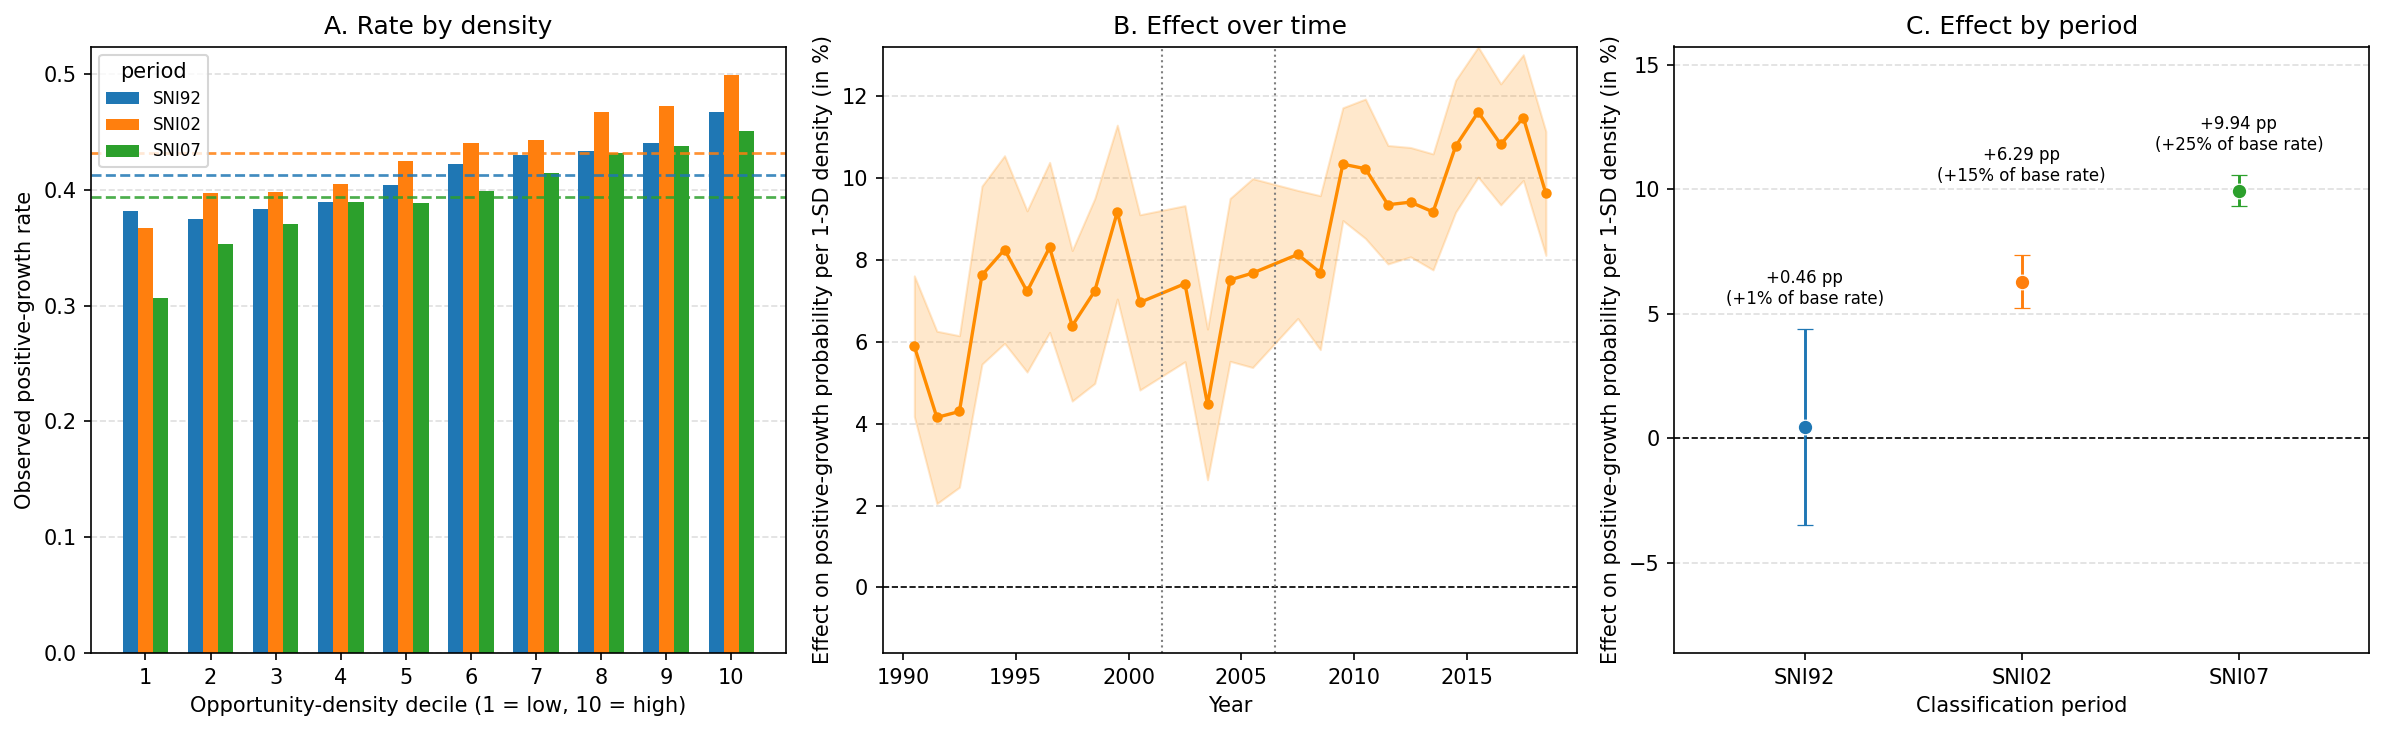
\includegraphics[width=\textwidth]{appendix/appendix_growth_binary.png}
\caption{\textbf{Opportunity density and positive employment growth.} The outcome equals one when industry employment increases between $t$ and $t+1$, among industries with positive employment in at least one of those years. Panel A shows observed probabilities by within-period opportunity-density decile; horizontal dashed lines show baseline rates. Panels B and C show year-specific and classification-period coefficients with 95\% confidence intervals, in percentage points per one-standard-deviation increase in the main opportunity density $D^{\mathrm{A,log}}$, using the standard deviation pooled across periods. Models include municipality$\times$year and industry fixed effects; year-specific coefficients come from density$\times$base-year interactions in the same model; standard errors are clustered by municipality and industry. Dotted vertical lines mark classification changes. Period sample sizes are 673,826, 260,664, and 922,960 for SNI92, SNI02, and SNI07. Any ``Effect'' or ``in \%'' labels in the supplied plot refer to associations in percentage points.}
\label{fig:si-growth-density}
\end{figure}

% REV006-S08: updated supplied figure, sample sizes, and estimator caption.
\begin{figure}[H]
\centering
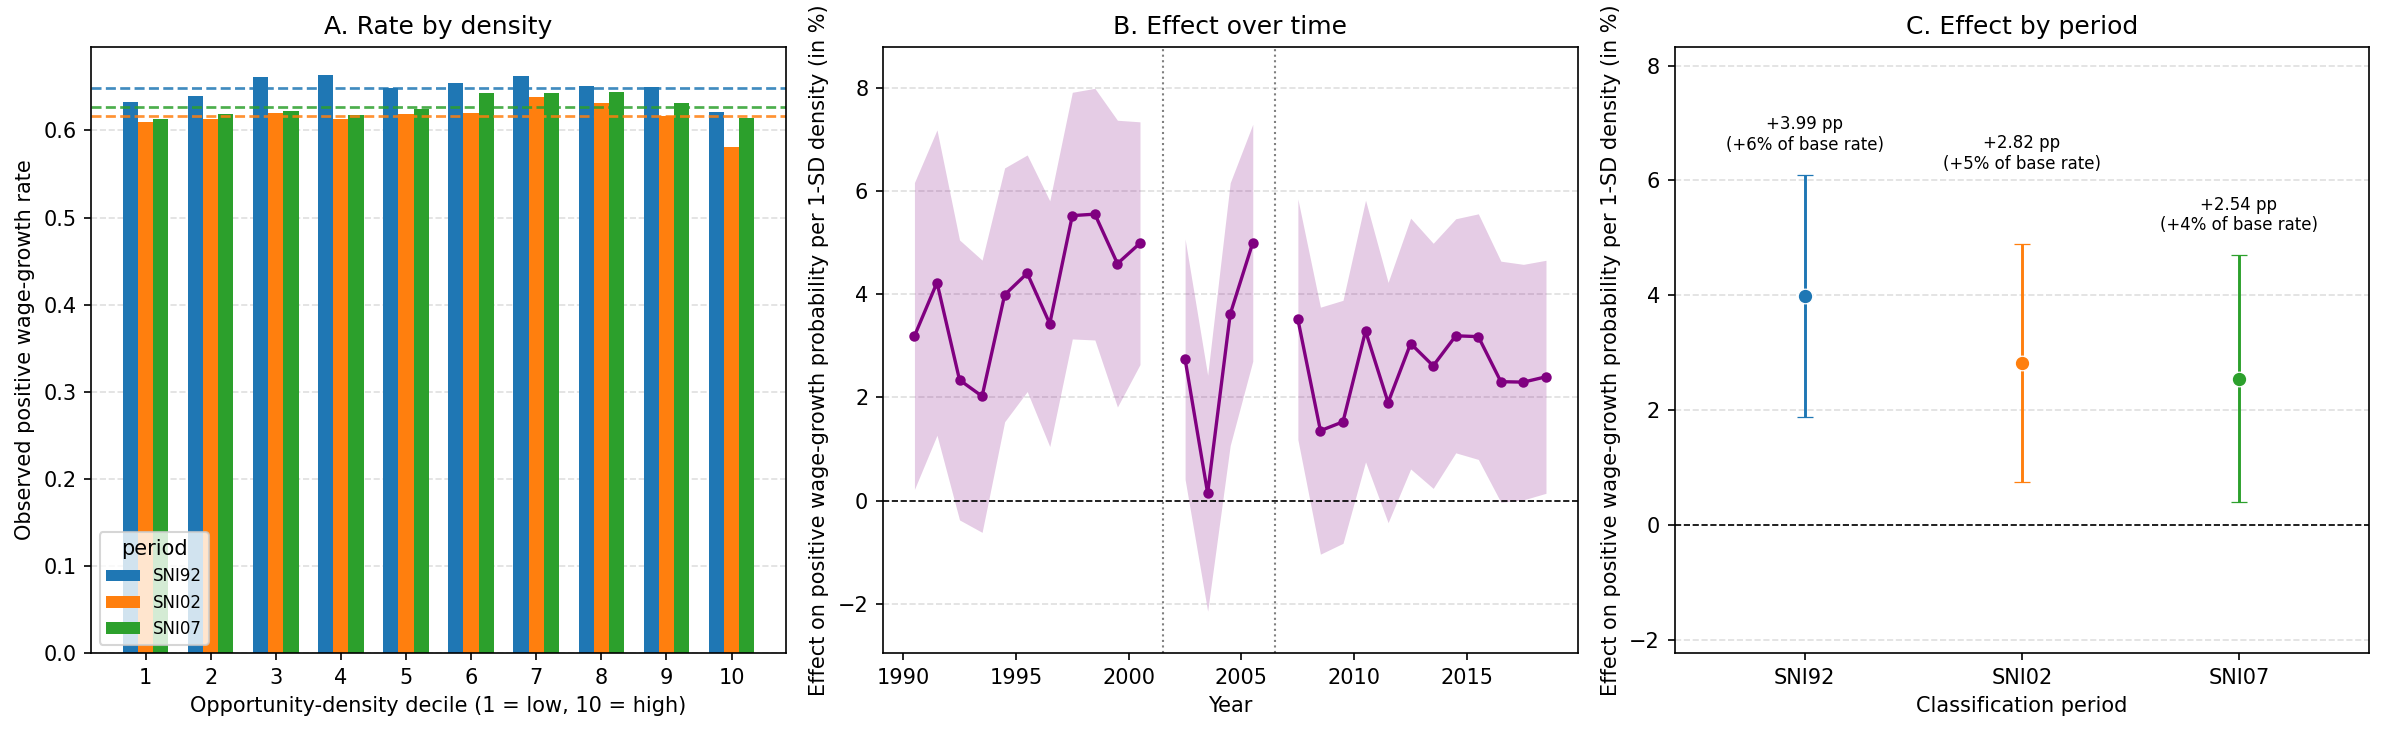
\includegraphics[width=\textwidth]{appendix/appendix_wage_growth_binary.png}
\caption{\textbf{Opportunity density and positive wage growth.} The outcome equals one when mean annual labour income rises between $t$ and $t+1$, among cells with more than five workers in both years. Panel A shows observed probabilities by within-period opportunity-density decile; horizontal dashed lines show baseline rates. Panels B and C show year-specific and classification-period coefficients with 95\% confidence intervals, in percentage points per one-standard-deviation increase in the main opportunity density $D^{\mathrm{A,log}}$, using the standard deviation pooled across periods. Models include municipality$\times$year and industry fixed effects; year-specific coefficients come from density$\times$base-year interactions in the same model; standard errors are clustered by municipality and industry. Dotted vertical lines mark classification changes. Period sample sizes are 366,937, 143,571, and 501,061 for SNI92, SNI02, and SNI07. Any ``Effect'' or ``in \%'' labels in the supplied plot refer to associations in percentage points.}
\label{fig:si-wage-growth}
\end{figure}

\clearpage
% REV006-S09: existing fixed-effects robustness figure, with corrected caption terminology.
\begin{figure}[H]
\centering
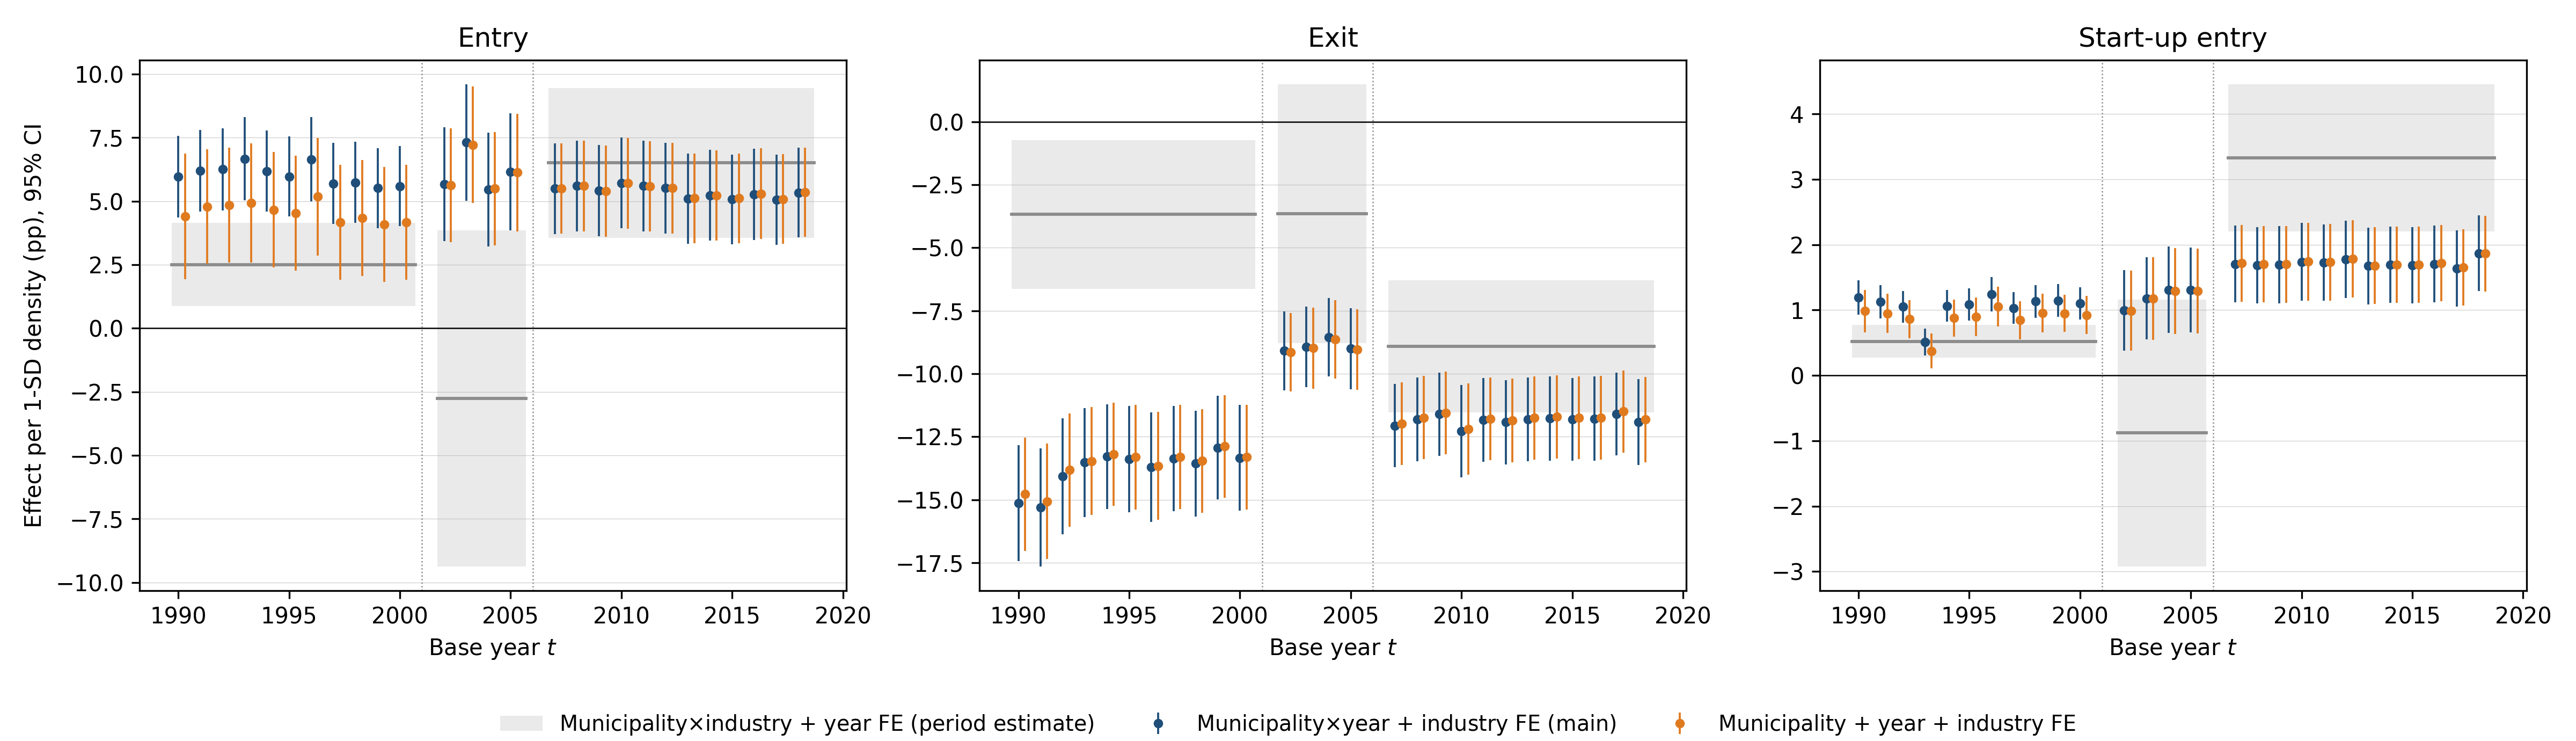
\includegraphics[width=\textwidth]{appendix/fe_robustness_annual.png}
\caption{\textbf{Opportunity-density associations under alternative fixed-effects specifications.} Year-specific coefficients in percentage points per one-standard-deviation increase in opportunity density, with 95\% confidence intervals, under the main specification (municipality$\times$year and industry fixed effects) and with additive municipality, year, and industry fixed effects. Grey bands show the period estimate and its 95\% confidence interval with municipality$\times$industry and year fixed effects. Density uses the standard deviation pooled across periods within each outcome. Standard errors are clustered by municipality and industry. Dotted lines separate the SNI92, SNI02, and SNI07 periods. These are single-density models; ``Start-up entry'' in the supplied plot denotes startup formation, and ``Effect'' denotes an association.}
\label{fig:fe_robustness_annual}
\end{figure}

% REV006-S10: main-specification multiple regressions for the growth outcomes.
\begin{figure}[H]
\centering
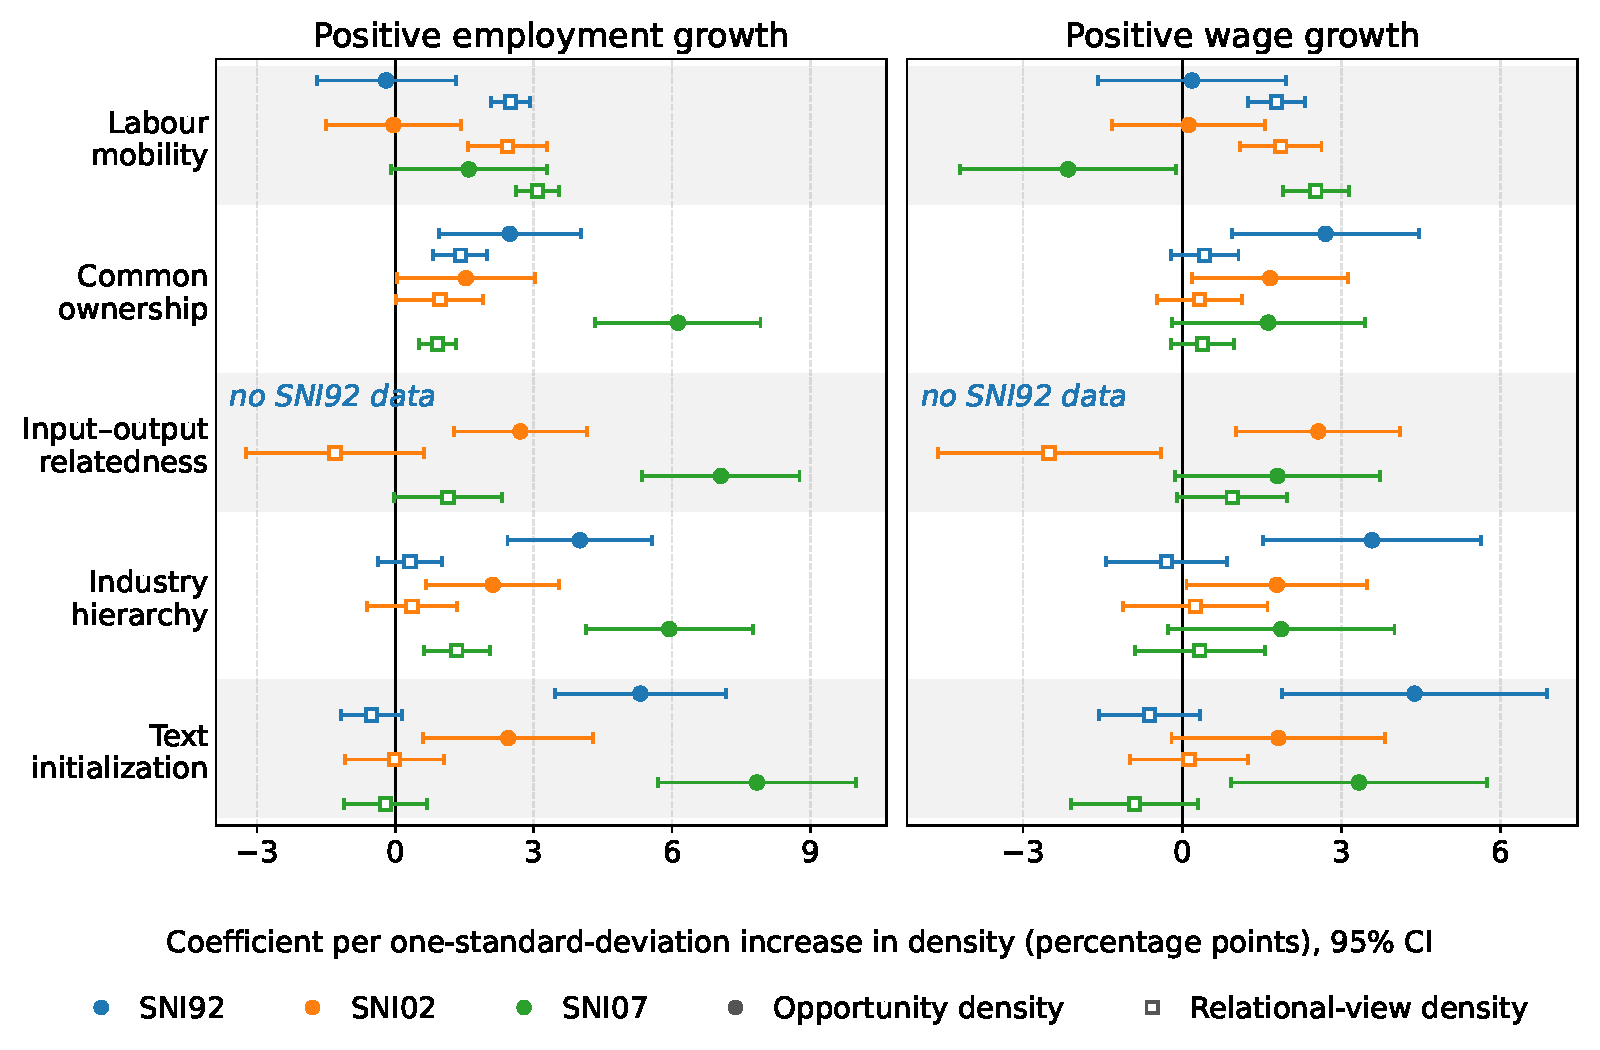
\includegraphics[width=\textwidth]{appendix/multiple_regression_growth.pdf}
\caption{\textbf{Opportunity density and relational-view densities in multiple regressions: employment and wage growth.} As Fig.~8 in the main text, for the probability of positive employment growth and positive wage growth. Each row and period shows one linear probability model with opportunity density (filled circles) and the density derived from one relational view or the untrained text initialization (open squares), with municipality$\times$year and industry fixed effects. Coefficients are percentage points per standard deviation of each density, standardized within the classification period; bars show 95\% confidence intervals with standard errors clustered by municipality and industry. Colours mark classification periods. Estimates are reported in Table~\ref{tab:multiple_regression_growth}; input--output relatedness is not available for SNI92.}
\label{fig:multiple-regression-growth}
\end{figure}

\clearpage
\SItext
\label{sec:methods}

We learn one shared latent representation from several relational views of industries. Each entity is an industry code in a particular classification version. Economic views describe labour mobility, common ownership, and input--output relatedness. Industry hierarchy and classification concordances provide additional constraints. All targets use the same cosine geometry, without source-specific projections of the embeddings.

Each relational view is encoded as a non-negative weighted graph on its relevant industry nodes. Row normalization gives a transition matrix, and graph diffusion produces scale-specific relational targets. Following semantic initialization, the shared industry embeddings are optimized against these targets and the ordinal hierarchy constraint. We assess reconstruction and classification fidelity, then combine latent proximity with regional employment portfolios to calculate opportunity density. Regional outcomes assess the empirical relevance of this proposed industrial-structural measure.

\subsection{Industry codes}
\label{subsec:industry-codes}

All relations are defined on Swedish Standard Industrial Classification (SNI) codes. We use SNI~1992 (SNI92), SNI~2002 (SNI02), and SNI~2007 (SNI07). Codes remain version-specific, so an identical digit string in two versions denotes two different entities. Each four-digit industry belongs to a three-digit group, a two-digit division, and a lettered section. The model contains 2,614 nodes: 1,634 four-digit industries and 980 hierarchy hubs. The four-digit counts are 505, 514, and 615 in SNI92, SNI02, and SNI07. Hub counts are 717 three-digit groups (222, 223, and 272), 208 divisions (60, 60, and 88), and 55 sections (17, 17, and 21).

Each code is a node in the graphs described below. Four-digit industries have independently learned embeddings; hubs are represented by their descendant means (Section~\ref{subsec:text-initialization}). Classification concordances link corresponding activities across adjacent versions while preserving version-specific entities.

\subsubsection{Labour mobility}
Labour mobility is measured using year-to-year transitions in linked employer–employee register data, following established approaches that identify industry changes from longitudinal worker records and exclude workers who remain in the same industry \cite{peterfrykblomMetodOchData2021,mondaniEvolvingNetworkLabor2017}. A move is counted only when both years fall inside the same classification period: 1990--2001 for SNI92, 2002--2006 for SNI02 and 2007--2019 for SNI07. Year pairs that straddle a change of classification are dropped, so that recoding is never read as an economic move, and workers who stay in the same four-digit industry are not
counted.

Within each period we first ask how many moves a pair of industries would be
expected to exchange given their size, growth and pay. Expected directed flows
are fitted by Poisson regression over all ordered pairs of industries,
including pairs with no observed move,
\begin{equation}
\begin{aligned}
\log \operatorname{E}[f_{ij}]
={}& \beta_0
+\beta_1 \log(1+e_i)
+\beta_2 \log(1+e_j) \\
&+\beta_3 g_i
+\beta_4 g_j \\
&+\beta_5 \log(1+y_i)
+\beta_6 \log(1+y_j).
\end{aligned}
\label{eq:expected-worker-flow}
\end{equation}
where $e$, $g$ and $y$ are an industry's mean employment (headcount), mean annual
employment growth (truncated to $[-0.9,3]$) and mean employment income over the period.
All coefficients are estimated without sign restrictions. Observed moves $f_{ij}$ are
then compared with expected moves, and the two directions are averaged,
\begin{equation}
r_{ij}=\frac{f_{ij}+1}{\widehat{\operatorname{E}}[f_{ij}]+1},
\qquad
\phi^{\mathrm{lab}}_{ij}=\tfrac{1}{2}\left(r_{ij}+r_{ji}\right).
\label{eq:labour-relatedness}
\end{equation}
The added ones keep the ratio finite for rare pairs. The directional-to-symmetric construction is consistent with prior labour-relatedness measures that first estimate $i\rightarrow j$ and $j\rightarrow i$ separately and then average the two normalized values \cite{elekesRegionalResilienceNetwork2024}

The use of observed flows relative to flows expected from industry characteristics follows the skill-relatedness literature, especially Neffke and Henning \cite{neffkeSkillRelatednessFirm2013}, who estimate expected directed labour flows using origin- and destination-industry size, growth, and wage characteristics

A pair is kept when the two directions together contain at least ten moves in the period. Because labour-flow matrices are sparse and relationships involving small industries are less precisely measured, prior studies impose minimum-flow thresholds or remove weak links before constructing the final network \cite{ocleryModularStructureLabour2022}.

\subsubsection{Common-ownership relations}
\label{subsubsec:common-ownership}

Common ownership is also measured between four-digit industries. For every
enterprise and year we list the distinct industries in which that enterprise
employs someone and count each pair of those industries once, regardless of how
many employees stand behind it. Enterprise-years covering more than 30
distinct industries are dropped before pairs are formed, since these are
typically umbrella identifiers that would otherwise link hundreds of unrelated
industries. Counts $c_{ij}$ are pooled over years within a classification
period and never across periods, and a pair is kept when it occurs in at least
three enterprise-years. The count is normalized by how often the two
industries co-occur with anything at all,
\begin{equation}
\phi^{\mathrm{own}}_{ij}=
\frac{c_{ij}+c_{ji}}
{c_{i\cdot}+c_{\cdot j}+c_{j\cdot}+c_{\cdot i}},
\label{eq:ownership-relatedness}
\end{equation}
where a dot denotes the sum over the corresponding row or column. Industries
that appear in many enterprises are therefore not treated as related to
everything.

\subsubsection{Input--output relations}
\label{subsubsec:input-output-relations}

Input--output relatedness is measured at the two-digit industry level, which corresponds to the effective resolution of the available symmetric input--output tables. We use three sources. For SNI07, we use Statistics Sweden's symmetric input--output tables for 2008--2016 and Sweden's observations in Eurostat's symmetric input--output dataset for 2010--2019. The Eurostat data are restricted to Sweden, domestic transactions, national-currency values, and product-to-product observations. For the pre-2008 period, we use Sweden's block from the 2013 release of the World Input--Output Database (WIOD) for 1995, 2000, and 2005. The WIOD release covers 1995--2011 and uses NACE Rev.1.1-style industries; in this project these observations are treated as SNI02-compatible. The source tables and their classifications are documented by Statistics Sweden, Eurostat, and WIOD \citep{statisticsswedenInputOutputTables2019,eurostat_suiot,timmerIllustratedUserGuide2015}.
The sources are retained in their native classification systems. SCB and Eurostat product codes are translated to SNI07 two-digit divisions, while WIOD industry codes are translated to SNI02 two-digit divisions. Aggregated source codes are expanded to the divisions they cover; for example, a code covering divisions 10--12 is mapped to 10, 11, and 12. When a source cell covers several origin and destination divisions, its value is divided equally across the resulting division pairs so that the total value is conserved. The implementation records the source-code translation and its audit table. No SNI92 input--output source is currently available, and WIOD observations are not crosswalked into SNI07 before relatedness is calculated.
For each source separately, flows are pooled across the listed years and converted into a symmetric flow-strength measure. Let \(f_{ij}\) denote the flow from division \(i\) to division \(j\), \(f_{i\cdot}\) its total outflow, and \(f_{\cdot i}\) its total inflow. We define
\begin{equation}
\phi^{\mathrm{io}}_{ij}=
\frac{f_{ij}+f_{ji}}
{f_{i\cdot}+f_{\cdot i}+f_{j\cdot}+f_{\cdot j}} .
\label{eq:io-relatedness}
\end{equation}
For pairs observed in both the SCB and Eurostat SNI07 tables, the source-specific values are averaged. The resulting input--output relations are stored separately as an SNI07 table, combining SCB and Eurostat, and an SNI02 table, based on WIOD. They are applied to two-digit SNI hub nodes in the graph; the procedure does not create direct four-digit input--output edges. The resulting two-digit input--output targets can nevertheless influence the four-digit embedding through the model's hub-aggregation step.

\subsubsection{Industry hierarchy}
The classification itself is a relation: within each classification version every four-digit
industry belongs to a three-digit group, every group to a two-digit division
and every division to a section. Each code is linked to its parent with weight
one, and the link is read in both directions. Hierarchy links never cross
classification versions. After the row normalization of
Equation~\eqref{eq:row-normalization}, a four-digit industry sends all of its
weight to its single parent, an intermediate code splits its weight evenly
between its children and its own parent, and a section splits its weight evenly
among its divisions.

\subsubsection{Classification concordances}
\label{subsubsec:cross-period-concordances}

Official concordances link four-digit codes of consecutive classifications, one
from SNI92 to SNI02 and one from SNI02 to SNI07. The two are built separately
and each is read in both directions. A code distributes a total weight of one
evenly over the codes it is mapped to: if code $i$ has $n_i$ listed
counterparts, each of those links receives weight $1/n_i$, and the same is done
from the newer code back to the older one. One-to-many and many-to-one
correspondences are thereby preserved, while a code with many counterparts does
not contribute more weight than a code with a single counterpart.

\subsubsection{Transition matrices and training targets}
\label{subsec:diffusion-targets}

Each empirical source defines a relation layer, indexed by $\ell$. The relation
may describe labour mobility, common ownership, input--output structure,
correspondence between two classification periods, or the industry hierarchy.
A layer is defined on a domain $D_\ell$, consisting of the industry codes to
which that source applies. Some layers generate multiple training targets when
they are evaluated at different diffusion depths.

For each relation layer $\ell$, let $W^{(\ell)}$ denote its non-negative
weighted adjacency matrix on domain $D_\ell$. Self-links are removed. We convert
this matrix into a row-normalized transition matrix,
\begin{equation}
P^{(\ell)}_{ij}
=
\frac{W^{(\ell)}_{ij}}
{\sum_{k\in D_\ell} W^{(\ell)}_{ik}},
\label{eq:row-normalization}
\end{equation}
for rows with positive outgoing weight. Thus, every non-zero row sums to one.
Rows without outgoing links remain zero and are excluded from the loss.

A training target is obtained by following the transitions in one relation
layer for $t$ steps:
\begin{equation}
P^{(\ell,t)}
=
\left(P^{(\ell)}\right)^t.
\label{eq:layer-diffusion}
\end{equation}
Here, $t=1$ represents direct relatedness, whereas larger values incorporate
paths through intermediate industries. Diffusion is performed separately
within each relation layer. When a layer is represented at multiple diffusion
depths, the resulting targets are retained separately rather than averaged.

The model uses seventeen training targets. Labour mobility
and the hierarchy are represented at $t=1$, $t=2$, and $t=4$, so that the
embedding captures both direct links and broader local connectivity. Worker
mobility contributes three scales for each of SNI92, SNI02, and SNI07. The
hierarchy contributes the same three scales across its classification levels.
The $t=1$ hierarchy target is replaced by an ordinal target defined only on
the SNI07 four-digit domain. The $t=2$ and $t=4$ hierarchy targets remain
categorical diffusion targets over the hub-inclusive hierarchy domain.

Common ownership is represented at $t=1$ and $t=4$ on the combined
block-diagonal graph of four-digit industries from all three classification
periods. The direct scale is the natural comparison for pairwise ownership,
while the additional $t=4$ target incorporates indirect ownership connections. The
input--output layer uses only $t=1$ at the two-digit level, matching the native
resolution of those tables. The SNI92--SNI02 and SNI02--SNI07 concordances also
use only $t=1$, because they encode direct one-to-one or one-to-many
classification transitions. Industry descriptions enter only through the semantic
initialization (Section~\ref{subsec:text-initialization}) and define no training target.

For the ordinal target, other industries are divided into four groups:
industries in the same three-digit group; industries in the same two-digit
division but a different three-digit group; industries in the same section but
a different two-digit division; and industries in a different section. For
each focal industry $i$, the objective encourages progressively lower
mean temperature-scaled cosine scores to these groups:
\begin{equation}
\overline{a}_{i,\mathrm{3d}}
>
\overline{a}_{i,\mathrm{2d}}
>
\overline{a}_{i,\mathrm{section}}
>
\overline{a}_{i,\mathrm{other}}.
\label{eq:hierarchy-order}
\end{equation}
A margin-ranking loss penalizes violations between neighboring groups, using a
margin of $0.05$.
For each row and each adjacent tier pair present in that row, the penalty is
$[0.05+\overline a_{i,\mathrm{farther}}-\overline a_{i,\mathrm{closer}}]_+$.
Penalties are averaged over valid adjacent tier pairs within a row, then over active rows.
The constraint acts on tier means, not on every individual industry pair, and uses no softmax.

\subsection{Learning the shared latent representation}
\label{subsec:learning-opportunity-space}

All relation layers are learned in a single shared latent space. We store one
64-dimensional vector for each of the $2,614$ nodes in the latent matrix
\begin{equation}
Z\in\mathbb{R}^{2614\times64},
\end{equation}
where $z_i$ denotes the row associated with node $i$. The rows corresponding to
four-digit industries are the model's free parameters. Higher-level nodes are
represented deterministically from these four-digit vectors before they are
used by any relation layer.

\subsubsection{Text-informed initialization and hierarchy aggregation}
\label{subsec:text-initialization}

Each node's official industry description is encoded once using the frozen
\texttt{sentence-transformers/all-MiniLM-L6-v2} model. The resulting
384-dimensional description embeddings are reduced to 64 dimensions using
principal-components analysis fitted on the descriptions of all $2,614$ nodes.
The reduced vectors are normalized to unit length and used to initialize the
rows of $Z$.

The language model remains frozen throughout relational training and does not
define a separate training objective. After initialization, only the rows of
$Z$ corresponding to four-digit industries are updated by the objectives
associated with the relation layers. The higher-level rows are not learned
independently. Instead, their effective representations are constructed from
their four-digit descendants at every forward pass.

For a higher-level node $a$, let $\mathcal{D}(a)$ denote the set of its
four-digit descendants in the same classification version. Its effective
representation is defined as the flat mean
\begin{equation}
\widetilde{z}_a
=
\frac{1}{|\mathcal{D}(a)|}
\sum_{i\in\mathcal{D}(a)} z_i,
\label{eq:hub-aggregation}
\end{equation}
whereas
\begin{equation}
\widetilde{z}_i=z_i
\end{equation}
for a four-digit industry $i$. The relation layers therefore operate on the
effective representations $\widetilde{z}$, while the independently learned
quantities are the four-digit vectors $z_i$.

Aggregation is performed directly over four-digit descendants rather than
recursively over intermediate hierarchy levels. Consequently, each four-digit
industry contributes equal weight to the representation of its three-digit
group, two-digit division, or section. Because higher-level representations are
functions of their descendants, gradients associated with a higher-level node
propagate to the four-digit vectors that define it.

\subsubsection{Shared-cosine observation model}
\label{subsec:shared-cosine}
We index individual training targets by $q$. Each target is associated with a
relation layer $\ell(q)$, a domain $D_q$, and, for categorical diffusion
targets, a transition depth $t_q$.
The latent similarity matrix has entries $S_{ij}(Z)=\cos(\widetilde z_i,\widetilde z_j)$. For each training target $q$, defined on domain $D_q$, the model assigns a
score to every pair of distinct nodes using the same shared latent
representation:
\begin{equation}
a^{(q)}_{ij}
=
\frac{\cos\left(\widetilde{z}_i,\widetilde{z}_j\right)}
{\tau_q},
\qquad
i,j\in D_q,\quad i\neq j.
\label{eq:cosine-score}
\end{equation}
The diagonal is masked so that a node cannot contribute to its own predicted
relatedness distribution. Each target has one learned positive temperature.
Let $\eta_q$ denote its unconstrained scalar parameter. The temperature is
defined as
\begin{equation}
\tau_q
=
\exp\left[
\operatorname{clip}(\eta_q,-1,1)
\right].
\label{eq:temperature}
\end{equation}
The model therefore uses no target-specific matrix, projection, or neural
scoring head. Target-specific differences enter only through the domain,
empirical target, loss, and temperature.

For categorical targets, the latent similarity distribution is obtained by applying a softmax over the
off-diagonal nodes in the target domain:
\begin{equation}
Q^{(q)}_{ij}
=
\frac{\exp\left(a^{(q)}_{ij}\right)}
{\displaystyle\sum_{k\in D_q\setminus\{i\}}
\exp\left(a^{(q)}_{ik}\right)},
\qquad
j\in D_q\setminus\{i\}.
\label{eq:predicted-distribution}
\end{equation}

For categorical targets, the diagonal of the empirical target is also removed.
Each target row is then renormalized over the same off-diagonal support used by
the prediction. Rows with no remaining target mass are excluded from the loss.

Labour-mobility, common-ownership, and input--output targets minimize the
row-wise Kullback--Leibler divergence,
\begin{equation}
\operatorname{KL}
\left(
P^{(q)}_i \,\middle\|\, Q^{(q)}_i
\right),
\end{equation}
averaged over active rows. The categorical hierarchy-diffusion and concordance
targets use cross-entropy. For a fixed target, raw KL and cross-entropy have identical gradients because target entropy is constant. Their numerical loss values differ, however, and affect baseline normalization, saturation, and dynamic reweighting. The ordinal hierarchy target instead uses the
margin-ranking loss defined in Equation~\eqref{eq:hierarchy-order}.

\subsubsection{Loss weighting and optimization}
\label{subsubsec:loss-weighting}

Raw losses are not directly comparable across targets with different domain
sizes or target entropies. Let \(b_q\) denote target \(q\)'s loss under a
trivial equal-score prediction over its admissible alternatives. An initial
family budget \(\lambda_{f(q)}\) is distributed among the targets belonging
to family \(f(q)\) in proportion to inverse null loss:
\begin{equation}
w^{(0)}_q
=
\lambda_{f(q)}
\frac{
b_q^{-1}
}{
\sum_{r:f(r)=f(q)}b_r^{-1}
}.
\label{eq:target-weight}
\end{equation}
This normalization guarantees that dividing a relational family into
multiple classification periods or diffusion depths does not mechanically
increase its initial total weight.

The initial family budgets in the selected specification are \(0.30\) for
labour mobility, \(0.25\) for input--output structure, \(0.125\) for common
ownership, \(0.10\) for the hierarchy, and \(0.10\) for the classification
concordances. These are starting loss weights rather than probabilities and
are subsequently adjusted by dynamic reweighting.

For target \(q\), let \(\mathcal{L}_{q,e}\) be its raw loss in epoch \(e\).
The implementation maintains an exponential moving average,
\begin{equation}
\overline{\mathcal{L}}_{q,e}
=
0.9\,
\overline{\mathcal{L}}_{q,e-1}
+
0.1\,
\mathcal{L}_{q,e},
\label{eq:loss-ema}
\end{equation}
initialized from the first-epoch loss. The dynamic reweighting ratio is
\begin{equation}
\rho_{q,e}
=
\min\left\{
\frac{
\overline{\mathcal{L}}_{q,1}
}{
\overline{\mathcal{L}}_{q,e}
},
20
\right\}.
\label{eq:dynamic-reweight}
\end{equation}
If this ratio would exceed \(2\), the loss must have improved by at least
\(10\%\) relative to its most recent stall reference. Otherwise, the ratio is
capped at \(2\) and the target is flagged as stalled.

The selected specification additionally applies a target-specific saturation
threshold equal to \(20\%\) of the null loss:
\begin{equation}
h_q=0.2b_q.
\label{eq:saturation-threshold}
\end{equation}
Below this threshold, the target contributes zero gradient in that epoch. Other targets and accumulated optimizer momentum can still move the shared embeddings. The joint loss in epoch \(e\) is therefore
\begin{equation}
\mathcal{L}_e
=
\sum_q
w^{(0)}_q
\rho_{q,e}
\left[
\mathcal{L}_{q,e}-h_q
\right]_+,
\label{eq:joint-loss}
\end{equation}
where \([x]_+=\max(x,0)\).

All target losses are computed from the same effective latent matrix in the
same forward pass. The embedding vectors and target-specific temperatures
are updated jointly with Adam for 500 full-batch epochs, using a learning
rate of \(10^{-2}\) and random seed 42. One joint backward pass and optimizer
step are performed per epoch. After training, the effective vectors are
normalized to unit length, and cosine similarity defines the common
shared latent geometry.

For a normalized categorical row, the derivative of raw KL or cross-entropy with respect to an off-diagonal score is $(Q^{(q)}_{ij}-P^{(q)}_{ij})/|\mathcal A_q|$, where $\mathcal A_q$ is the set of active rows. Connections assigned more target probability than predicted probability contribute pressure to increase their scores. The reverse contributes pressure to decrease scores. These contributions are combined across targets, scaled by effective weights, and passed through saturation. Shared embedding vectors couple the pairwise comparisons, so targets can exert competing gradients.

Let $H$ be the fixed matrix that averages four-digit descendants for each hub. Writing the effective embedding matrix as $U=HZ$, hub gradients reach the four-digit parameters through $H^{\mathsf T}(\partial\mathcal L/\partial U)$. Gradients also pass through cosine normalization and each target's learned log-temperature. The clamp in the temperature transformation has zero derivative outside its permitted interval. Dynamic weights are calculated from detached scalar losses and are treated as constants during each backward pass. The target matrices, domain masks, diffusion calculations, text encoder, PCA, and hub aggregation remain fixed. Training exports the final parameter state; no checkpoint is selected by loss.


\subsection{Evaluation of the shared latent representation}
\label{subsec:embedding-evaluation}

We evaluate the learned representation along three dimensions: reconstruction
of the constituent relational evidence, preservation of the official
classification structure, and alignment across successive classification
periods.

Reconstruction of labour-mobility and common-ownership relatedness is measured
by the Spearman correlation between observed pairwise relatedness and cosine
similarity in the learned representation, separately for SNI92, SNI02, and
SNI07. Input--output reconstruction is evaluated for SNI07 at the two-digit
division level in two ways. First, we correlate input--output relatedness with
cosine similarity between the corresponding effective two-digit aggregate
vectors. Second, we correlate input--output relatedness with the mean cosine
similarity across all pairs of four-digit industries belonging to the two
divisions.

Cross-version alignment is evaluated as a retrieval problem for the SNI92 to
SNI02 and SNI02 to SNI07 concordances. For every source code, all codes in
the subsequent classification are ranked by cosine similarity. Because a
source code can have multiple valid successors, we report mean reciprocal
rank, mean average precision over the complete set of valid successors, and
\(\mathrm{Hit@}k\) for
\[
k\in\{1,5,10,20\}.
\]
In this implementation, \(\mathrm{Hit@}k\) equals one for a source code
when at least one valid successor occurs among its first \(k\) retrieved
codes and zero otherwise.

Preservation of the official hierarchy is evaluated for SNI07 four-digit
industries. We compare cosine similarities between industries belonging to
the same three-digit group, the same two-digit division but different
three-digit groups, the same section but different two-digit divisions, and
different sections. Ordinal preservation is summarized by the Spearman
correlation between cosine distance and the resulting four-level
classification-tree distance (1 for the same three-digit group to 4 for different
sections). Because 82\% of the 188,805 SNI07 pairs lie in different sections, the
correlation is computed on pairs balanced across the four tiers: all 865
same-group pairs and all 3,594 same-division pairs, plus 5,000 same-section and
5,000 different-section pairs drawn at random with seed 42 (14,459 pairs).
Same-section pairs are drawn by selecting a section at random and then two of its
industries from different divisions; draws are independent, so a pair can recur.
The same design is applied to the text-encoder baseline. Mean similarities by tier
use all pairs. We also calculate the cosine-distance
silhouette score of SNI07 sections.

All quantitative results use the original cosine geometry. The cosine-distance silhouette for SNI07 sections is $-0.0461$, indicating that these sections do not form globally separated clusters in the learned representation. A two-dimensional projection is not used to calculate opportunity density.

For comparison, the same evaluation metrics are computed using the original
384-dimensional, normalized
\texttt{sentence-transformers/all-MiniLM-L6-v2} description embeddings. This
text-only baseline uses the same encoder and industry descriptions that
provide the initialization of the learned representation. It is not subjected
to the subsequent 64-dimensional principal-components projection. Differences
between the baseline and learned representation therefore reflect both the
dimensionality reduction and the subsequent relational optimization.

% REV009-S02: the regional evaluation is complemented by hold-out checks.
Labour mobility, common ownership, input--output structure, the hierarchy,
and classification concordances all contribute to model fitting. Their
reconstruction, hierarchy, and retrieval statistics should therefore be
interpreted as transductive fidelity diagnostics rather than as independent
or out-of-sample validation. Regional outcomes provide a downstream assessment of empirical relevance. They are excluded from the training objective, but some training inputs derive from overlapping register data. Section~\ref{subsubsec:holdout} therefore re-estimates the regional models with representations trained without the evaluated municipalities or years.

\subsubsection{Regional employment panel}
\label{subsubsec:regional_employment_panel}

The regional employment panel is constructed from individual-level employment
records for 1990--2019. Each individual is assigned to the municipality and
four-digit industry of their workplace. We aggregate these observations to
obtain employment
\[
E_{mjt},
\]
where \(E_{mjt}\) denotes the number of workers employed in industry \(j\), in
municipality \(m\), in year \(t\).

Municipal identifiers are harmonized over time using a municipality
crosswalk. Industry codes are evaluated within three classification periods:
SNI92 for explanatory years 1990--2000, SNI02 for 2002--2005, and SNI07 for
2007--2018. Outcomes are measured in year \(t+1\), so the corresponding outcome
years extend through 2001, 2006, and 2019, respectively. Observations with
missing or invalid municipality or industry identifiers are excluded.

\subsubsection{Construction of entry and exit variables}
\label{subsubsec:regional_entry_exit}

Entry and exit are defined on classification-specific
municipality--industry panels. Because very small employment observations may
reflect marginal or transitory activity, we distinguish economically
meaningful regional industry activity using the distribution of industry
employment within each municipality and year.

For every active industry \(i\) in municipality \(m\) and year \(t\), we
transform employment as
\[
A_{mit}=\operatorname{asinh}(E_{mit}).
\]
Let
\[
\mathcal{A}_{mt}=\{i:E_{mit}>0\}
\]
be the set of active industries in the municipality. We calculate
\[
\overline{A}_{mt}
   =\frac{1}{|\mathcal{A}_{mt}|}
      \sum_{i\in\mathcal{A}_{mt}}A_{mit}
\]
and the corresponding population standard deviation
\[
\sigma_{mt}
   =
   \left[
   \frac{1}{|\mathcal{A}_{mt}|}
   \sum_{i\in\mathcal{A}_{mt}}
   \left(A_{mit}-\overline{A}_{mt}\right)^2
   \right]^{1/2}.
\]
A municipality--industry observation is classified as meaningful activity
when
\[
Q_{mjt}
 =
 \mathbf{1}\left\{
 E_{mjt}>0,\quad
 \overline{A}_{mt}-2\sigma_{mt}
 \leq A_{mjt}\leq
 \overline{A}_{mt}+2\sigma_{mt}
 \right\}.
\]
The activity band is only defined for municipality--years containing at least
two active industries and a positive within-municipality standard deviation.

The risk set for industry entry contains industries that are absent from a
municipality in year \(t\):
\[
\mathcal{R}^{\mathrm{entry}}_t
 =
 \{(m,j):E_{mjt}=0\}.
\]
The entry outcome is
\[
Y^{\mathrm{entry}}_{mjt+1}
 =
 Q_{mjt+1},
 \qquad
 (m,j)\in\mathcal{R}^{\mathrm{entry}}_t.
\]
Thus, an entry occurs when an industry that was absent in year \(t\) exhibits
meaningful employment in year \(t+1\).

The exit risk set contains industries that are present in year \(t\):
\[
\mathcal{R}^{\mathrm{exit}}_t
 =
 \{(m,j):E_{mjt}>0\}.
\]
The exit outcome is
\[
Y^{\mathrm{exit}}_{mjt+1}
 =
 Q_{mjt}\,
 \mathbf{1}\{E_{mjt+1}=0\},
 \qquad
 (m,j)\in\mathcal{R}^{\mathrm{exit}}_t.
\]
This definition restricts exits to industries with meaningful activity before
their disappearance. These definitions adapt the broader regional-diversification approach of studying changes in local activity presence
\cite{hidalgoProductSpaceConditions2007,boschmaRelatednessDriverRegional2017}.

\subsubsection{Identification of startups}
\label{subsubsec:regional_startups}

Startup formation is identified by combining the individual employment records
with establishment-demography information. Employment records are first
aggregated by organization number and year. A candidate startup must satisfy
the following conditions: the organization number is not observed in the
immediately preceding year; the organization operates a single establishment;
and its initial employment is no greater than ten workers.

Candidate organizations are then matched to the establishment-demography
records using organization number, establishment number, and year. We retain
demographic event codes \(1\), \(2\), \(3\), \(6\), \(7\), and \(8\), while
excluding events classified as mergers or continuations of existing
organizations. The currently implemented specification does not impose an
additional employment-growth filter.

Organizations meeting these criteria are aggregated to the
municipality--industry--founding-year level. Let \(S_{mjt}=1\) indicate that
at least one such organization is founded in municipality \(m\) and
industry \(j\) in year \(t\). Startup formation is evaluated among industries
that are absent from the municipality in the preceding year:
\[
Y^{\mathrm{startup}}_{mjt+1}
 =
 S_{mjt+1},
 \qquad
 (m,j)\in\mathcal{R}^{\mathrm{entry}}_t.
\]
The variable therefore measures the entry of a new industry through startup
formation, rather than subsequent startup growth. The construction is
oriented toward established approaches to identifying new firms and their role
in regional diversification
\cite{anderssonCharacteristicsPerformanceNew2013,
grillitschDoesTimingIntegrating2021}.

\subsubsection{Opportunity density}
\label{subsubsec:regional_opportunity_density}

Let \(\mathbf{z}_j\) denote the learned unit-normalized embedding of industry
\(j\) in the shared latent representation. Latent proximity between industries \(i\) and \(j\) is measured by cosine similarity:
\[
c_{ij}
 =
 \mathbf{z}_i^{\mathsf T}\mathbf{z}_j.
\]
Opportunity density measures how aligned a candidate industry is on average to all other industries already present in the municipality. The focal
industry is excluded from its own density calculation.

In the main specification, density is the log-employment-weighted arithmetic
mean of the similarity between industries:
\[
D^{\mathrm{A,log}}_{mjt}
 =
 \frac{
   \sum_{i\neq j}W^{\log}_{mit}c_{ij}
 }{
   \sum_{i\neq j}W^{\log}_{mit}
 },
 \qquad
 W^{\log}_{mit}=\log(1+E_{mit}).
\]
Log-transforming employment before weighting dampens the influence of the
largest regional industries relative to a raw employment weight, so that
the measure gives less weight to a few very large industries.

We examine three alternative constructions as robustness checks: the
employment-weighted arithmetic mean using raw (untransformed) employment,
\[
D^{\mathrm{A}}_{mjt}
 =
 \frac{
   \sum_{i\neq j}E_{mit}c_{ij}
 }{
   \sum_{i\neq j}E_{mit}
 },
\]
and the corresponding weighted geometric means. Because cosine similarity can
be negative, similarities are first mapped to the unit interval:
\[
s_{ij}
 =
 \max\left\{
 \frac{c_{ij}+1}{2},\epsilon
 \right\},
\]
where \(\epsilon=10^{-12}\). Geometric density under weight \(W_{mit}\)
(raw \(E_{mit}\) or log-transformed \(W^{\log}_{mit}\)) is then
\[
D^{\mathrm{G}}_{mjt}
 =
 \exp\left[
 \frac{
   \sum_{i\neq j}W_{mit}\log(s_{ij})
 }{
   \sum_{i\neq j}W_{mit}
 }
 \right].
\]
% REV006-S11: significance level and outcome-specific pooled scaling.
Combining the arithmetic or geometric aggregation rule with raw or
log-transformed employment produces four density specifications. The
log-employment-weighted arithmetic mean, \(D^{\mathrm{A,log}}\), is the main
specification used throughout; the raw-employment arithmetic mean, the
raw-employment geometric mean, and the log-employment geometric mean are
robustness specifications. Across the entry, exit, and startup formation
outcomes, all four specifications yield coefficients of the same sign and
statistically significant at the 1\% level (Table~\ref{tab:density_robustness}). Log-weighting changes coefficient magnitudes without changing their signs; it does not increase every coefficient under every aggregation rule.

Before estimation of the main models, density is scaled by its standard deviation over the pooled
regional evaluation panel of each outcome, across all three classification periods:
\[
D^{*}_{mjt}
 =
 \frac{D_{mjt}}{\operatorname{SD}(D)}.
\]
When the main arithmetic measure has zero total weight on other industries, the implementation returns zero. This is a computational convention, not evidence that opportunity is absent. For the geometric variants, the same empty-weight case returns one.

The variable is not mean-centered. A one-unit increase in \(D^{*}_{mjt}\)
therefore corresponds to a one-standard-deviation increase in opportunity
density. The multiple regressions in Section~\ref{subsubsec:multiple-regression} instead divide each density by its own within-period standard deviation.

% REV006-S12: exact absorption, singleton removal, two-way inference, annual interactions.
\subsubsection{Regression design}
\label{subsubsec:regional_regression}

For each outcome $k$ (industry entry, industry exit, or startup formation) and classification period, we estimate linear probability models
\begin{equation}
Y^{k}_{mj,t+1}=\beta^{k}D^{*}_{mjt}+\alpha_{mt}+\gamma_j+\varepsilon^{k}_{mj,t+1},
\label{eq:si-regional-main}
\end{equation}
with municipality$\times$year fixed effects $\alpha_{mt}$ and industry fixed effects $\gamma_j$. Municipality$\times$year effects absorb everything that varies at the level of a municipality in a given year, such as total employment, the number of active industries, and local business cycles. The coefficient $\beta^k$ is identified from differences in density across industries within the same municipality and year, after accounting for persistent industry differences. Each classification period is estimated separately because code strings overlap across versions but denote different industries.

The risk sets are unbalanced: entry and startup formation are defined for industries absent from a municipality in year $t$, and exit for industries present. Singleton observations, which are alone in a fixed-effect group, are removed iteratively. Outcome and density are then residualized on both sets of fixed effects by alternating projections. Iteration stops when the largest absolute group-mean correction, scaled by the original standard deviation of its variable (with a floor of $10^{-12}$), is below $10^{-10}$. The coefficient is the least-squares coefficient of the residualized outcome on residualized density.

Opportunity density depends on each industry's position in the latent space, motivating allowance for residual dependence across municipalities for the same industry as well as within municipalities. Standard errors are clustered by municipality and industry~\cite{cameronRobustInferenceMultiway2011}, using
\[
V=V_{\mathrm{municipality}}+V_{\mathrm{industry}}-V_{\mathrm{municipality}\cap\mathrm{industry}},
\]
with a $G/(G-1)$ small-sample factor for each component, where $G$ is the number of clusters in that component. The implementation symmetrizes the covariance estimate and clips negative eigenvalues to zero. Confidence intervals and $p$-values use a $t$ distribution with $\min(G_{\mathrm{municipality}},G_{\mathrm{industry}})-1$ degrees of freedom (288 or 289 in these analyses); $p$-values below 0.001 are reported as $p<0.001$.

Year-specific coefficients are estimated in the same model by replacing $D^{*}_{mjt}$ with its interactions with base-year indicators. They use the same fixed effects and clustering as the period estimate. Table~\ref{tab:regional-samples} gives sample sizes after singleton removal, baseline outcome rates, and period estimates.

Because the dependent variable is binary, $\beta^k$ is reported as an association with the probability of the outcome, in percentage points ($100\beta^k$). To express its magnitude relative to the rarity of the outcome, we divide it by the observed baseline rate within the corresponding risk set and period:
\[
\overline{Y}^{k}_{r}=\frac{1}{N_r}\sum_{(m,j,t)\in r}Y^{k}_{mj,t+1},
\qquad
100\times\frac{\beta^{k}_{r}}{\overline{Y}^{k}_{r}}.
\]
For example, a coefficient of $0.03$ and a baseline rate of $0.05$ correspond to a three-percentage-point association, or $60\%$ of the observed baseline rate. The coefficient-to-baseline ratio is a scale comparison, not a relative risk or a causal percentage change; a ratio below $-100\%$ does not imply a negative event probability.

% REV009-S03: new subsection, hold-out and training stability (Tables S4--S6).
\subsubsection{Spatial and temporal hold-out and training stability}
\label{subsubsec:holdout}

The relational views and the regional outcomes partly derive from the same register data. To assess whether the associations depend on this overlap, we retrain the representation without the municipalities or years in which density is evaluated. All other training settings remain unchanged, and the candidate panels, outcomes, and density formula are those of the main models. Only the representation from which cosine similarities are taken changes.

\textit{Spatial hold-out.} The 290 municipalities are grouped into quintiles of mean annual workplace employment (1990--2019) and assigned at random within each quintile to five folds of 58 municipalities; Stockholm, Gothenburg, and Malmö are placed in different folds. For each fold, labour mobility and common ownership are rebuilt after removing every person-year whose workplace lies in the fold, and the representation is retrained. Input--output relatedness is national and remains unchanged. Workplace codes that cannot be assigned to a municipality (0.25\% of employed person-years) are retained in every fold. The density of each municipality is then calculated from its own employment and the representation that excluded it. Each of the five representations implies its own density level for every industry. With a common industry fixed effect, these level differences would remain in the regressor as noise unrelated to the outcomes and bias the coefficient towards zero. The pooled models therefore include municipality$\times$year and industry$\times$fold fixed effects. Because each municipality belongs to one fold, all fixed effects are then fold-specific, and the coefficient is a precision-weighted combination of the coefficients within the five folds. Applied to the reported representation, this specification changes the coefficients by at most $0.16$ percentage points (Table~\ref{tab:holdout-spatial}). The procedure is repeated for three random fold assignments.

\textit{Temporal hold-out.} For $T_0=2015$, $2016$, $2017$, and $2018$, the representation is retrained on labour mobility restricted to moves up to $T_0-1\rightarrow T_0$, common ownership up to $T_0$, and input--output tables with source years up to $T_0$. In the hold-out test, density in explanatory year $T_0+1$ is related to outcomes in $T_0+2$ ($T_0=2015$--$2017$), so neither the employment underlying the density nor the outcomes entered training. The three explanatory years 2016--2018 of the SNI07 period are estimated jointly with year-specific coefficients and industry$\times$year fixed effects, for the reason given above. In a second test, density in $T_0$ is related to entry and exit $h=1$, $2$, or $3$ years later, with the definitions of the main models applied between $T_0$ and $T_0+h$ (startup formation: $h=1$ only). Windows are pooled with industry$\times T_0$ fixed effects. In both tests, the reported representation is estimated with the same specification on the same observations.

\textit{Training stability.} Full-batch training from the text initialization involves almost no randomness, so changing the random seed alone hardly changes the result. We therefore perturb the initialization: Gaussian noise with variance $0.5^2/64$ per dimension is added to each normalized initial vector before renormalization, giving a mean cosine similarity of $0.90$ with the unperturbed initialization. Ten representations are trained from independent perturbations. Training is deterministic on a given machine but not bitwise reproducible across machines; we therefore also retrain the reported representation without perturbation.

\textit{Results.} In the spatial hold-out, the coefficients are $76$--$90\%$ of the main estimates for industry entry, $101$--$103\%$ for industry exit, and $82$--$92\%$ for startup formation, all with $p<0.01$ and with the same conclusions for all three fold assignments (Table~\ref{tab:holdout-spatial}). Estimated separately for the 58 municipalities of each fold, 42 of 45 entry coefficients, 43 of 45 startup-formation coefficients, and all exit coefficients have the sign of the main estimates. In the temporal hold-out, the coefficients are $77\%$, $97\%$, and $75\%$ of the main estimates on the same observations (Table~\ref{tab:holdout-temporal}). The year-specific confidence intervals exclude zero except for startup formation in 2017 ($0.75$ percentage points, 95\% CI $-0.12$ to $1.62$). Over longer horizons, the hold-out coefficients grow with $h$, as do those of the main representation, and remain at $75$--$98\%$ of them. Across perturbed initializations, the standard deviation of the coefficients is at most $0.17$ percentage points and less than a fifth of their standard errors (Table~\ref{tab:holdout-seeds}). The evaluation metrics of the representation vary as little: across the ten runs, the labour-mobility and common-ownership correlations for SNI07 are $0.565\pm0.003$ and $0.694\pm0.003$ (mean $\pm$ SD; reported representation $0.562$ and $0.694$), the input--output correlation is $0.910\pm0.0004$, the hierarchy correlation $0.374\pm0.002$, and SNI02-to-SNI07 Hit@1 $0.715\pm0.012$. The ten nearest neighbours of an SNI07 industry overlap with a mean Jaccard index of $0.85$ between runs, and pairwise cosine similarities correlate at $0.98$.

% REV006-S13: main-specification multiple regressions replace single-source correlations.
\subsubsection{Multiple regressions with relational-view densities}
\label{subsubsec:multiple-regression}

To assess whether opportunity density carries information beyond the individual relational views, we construct a density for each view with the same formula as $D^{\mathrm{A,log}}$ (log-employment weights, focal industry excluded), replacing the cosine similarity $c_{ij}$ with the view's relation between industries $i$ and $j$:
\begin{itemize}
\item Labour mobility and common ownership: the row-normalized transition matrices $P^{(\ell)}_{ij}$ of Eq.~\eqref{eq:row-normalization} used in training, so that the density of $j$ sums the shares of local industries' relatedness directed towards $j$.
\item Input--output relatedness: $\phi^{\mathrm{io}}$ for the industries' two-digit divisions for pairs in different divisions, with zero within a division; no SNI92 source is available.
\item Industry hierarchy: 3 for the same three-digit group, 2 for the same division but different groups, 1 for the same section but different divisions, and 0 otherwise.
\item Text initialization: cosine similarity of the untrained 64-dimensional PCA initialization (Section~\ref{subsec:text-initialization}).
\end{itemize}
All densities are computed on the same candidate panels as the main analysis. For each outcome, classification period, and view $V$, we estimate
\begin{equation}
Y^{k}_{mj,t+1}=\beta^{k}_{O}D^{O*}_{mjt}+\beta^{k}_{V}D^{V*}_{mjt}+\alpha_{mt}+\gamma_j+\varepsilon^{k}_{mj,t+1},
\label{eq:si-regional-multiple}
\end{equation}
where $D^{O*}$ is opportunity density and $D^{V*}$ the view's density, each divided by its standard deviation within the period, with the fixed effects, estimation, and clustering of Section~\ref{subsubsec:regional_regression}. The coefficient $\beta^{k}_{O}$ measures the association of opportunity density holding the view's density constant, and vice versa. Each density uses its own standard deviation, so differences in coefficient size between densities describe their respective scales. This within-period scaling also differs from the pooled scaling of the main models; changes in coefficient magnitude across these analyses cannot be attributed solely to including the second density.

The models are estimated for industry entry, industry exit, and startup formation (main text, Fig.~8; Table~\ref{tab:multiple_regression}) and for positive employment and wage growth (Section~\ref{subsec:growth}; Fig.~\ref{fig:multiple-regression-growth}; Table~\ref{tab:multiple_regression_growth}). The main-text statement that opportunity density remains associated in 41 of 42 models refers to its 95\% confidence interval excluding zero in the models in Table~\ref{tab:multiple_regression}. The exception is industry entry in SNI07 with labour-mobility density ($1.80$ percentage points; 95\% CI $-0.15$ to $3.75$). These intervals are pointwise and are not adjusted for multiple comparisons.

% REV006-S14: fixed-effects robustness concerns single-density models only.
\subsubsection{Fixed-effects specification and inference}
\label{subsubsec:fe-robustness}

Table~\ref{tab:fe_robustness} compares the main specification with additive municipality, year, and industry fixed effects and with municipality$\times$industry and year fixed effects. All three specifications use the estimation and two-way clustering described in Section~\ref{subsubsec:regional_regression}. These robustness models include opportunity density as the sole density regressor. Figure~\ref{fig:fe_robustness_annual} shows year-specific coefficients for the main and additive specifications, together with period estimates for the municipality$\times$industry specification.

The additive specification gives estimates close to the main specification in SNI02 and SNI07. In SNI92, industry-entry and startup-formation coefficients are smaller ($4.58$ versus $6.05$ and $0.87$ versus $1.05$ percentage points), with overlapping confidence intervals. Their signs and the conclusion of positive associations are retained. Overlapping intervals do not by themselves establish equivalence between specifications.

Municipality$\times$industry fixed effects identify the coefficient from changes in density over time within a municipality--industry cell, net of common year effects. The eligible observations can change when an industry enters or exits, and singleton removal also changes the estimation sample. In SNI92 and SNI07 the coefficients retain their signs and their confidence intervals exclude zero. For SNI07, the entry and startup-formation coefficients are larger than in the main specification ($6.51$ and $3.33$ percentage points) and the exit coefficient is smaller in magnitude ($-8.91$). For SNI92 all three magnitudes are smaller (entry $2.51$, exit $-3.68$, startup formation $0.52$). In SNI02, which covers four base years, all three intervals include zero. These estimates therefore qualify the precision of associations identified from within-cell changes in that period. Figure~\ref{fig:fe_robustness_annual} reports period estimates for this specification rather than year-specific coefficients.

% REV006-S15: binary growth results and their conditional boundary; softmax analysis removed.
\subsection{Employment and wage growth}
\label{subsec:growth}

Employment growth is $\operatorname{asinh}(E_{mj,t+1})-\operatorname{asinh}(E_{mjt})$, evaluated for industries with positive employment in at least one of $t$ and $t+1$. Wage growth is the change in the inverse hyperbolic sine of mean annual labour income, evaluated for cells with more than five workers in both years. The outcomes equal one when the respective growth measure is positive. The employment-growth sample therefore also includes cells where employment appears or disappears; it is not restricted to industries present in both years. We relate these outcomes to the main opportunity density $D^{\mathrm{A,log}}$ using the regression design of Section~\ref{subsubsec:regional_regression} (Figs.~\ref{fig:si-growth-density} and \ref{fig:si-wage-growth}) and the multiple regressions of Section~\ref{subsubsec:multiple-regression} (Fig.~\ref{fig:multiple-regression-growth}; Table~\ref{tab:multiple_regression_growth}).

Opportunity density is associated with a higher probability of positive employment growth: $5.22$ percentage points in SNI92 (95\% CI $3.50$--$6.95$), $3.53$ in SNI02 ($1.57$--$5.48$), and $8.21$ in SNI07 ($6.42$--$9.99$; all $p<0.001$). These coefficients correspond to $8$--$21\%$ of baseline rates. Positive wage-growth associations are $3.99$ percentage points in SNI92 (95\% CI $1.88$--$6.10$; $p<0.001$), $2.82$ in SNI02 ($0.74$--$4.89$; $p=0.008$), and $2.54$ in SNI07 ($0.39$--$4.70$; $p=0.021$), or $4$--$6\%$ of baseline rates.

None of the opportunity-density coefficients retains a positive association with a 95\% confidence interval excluding zero once labour-mobility density is included. The opportunity-density coefficients for employment growth ($-0.20$, $-0.04$, $1.59$) and for wage growth in SNI92 and SNI02 ($0.18$, $0.12$) have intervals including zero. The wage-growth coefficient in SNI07 is negative ($-2.15$; 95\% CI $-4.19$ to $-0.11$), whereas labour-mobility density remains positive with intervals excluding zero throughout (Fig.~\ref{fig:multiple-regression-growth}; Table~\ref{tab:multiple_regression_growth}). Labour mobility thus retains an association with these growth outcomes after opportunity density is accounted for. The main text focuses on industry entry, industry exit, and startup formation.

% REV006-S16: distinguish text initialization in multiple regressions from the encoder baseline.
\subsection{Evaluation KL and the text baselines}
The source-wise evaluation KL values in Table~\ref{tab:source-period-metrics} use a fixed cosine-softmax temperature of $\tau=0.05$. They are separate diagnostics, not the target-specific optimized training losses. Training learns a distinct temperature for each target within $[\exp(-1),\exp(1)]$. The reconstruction and retrieval baseline is the original 384-dimensional text encoder. In the multiple regressions of Section~\ref{subsubsec:multiple-regression}, the text initialization is the untrained 64-dimensional PCA semantic initialization. No language-model parameters are fine-tuned.

\clearpage
% REV006-S17: new bibliography supplement; original references.bib preserved.
\bibliography{references}
\end{document}
